%%%%%%%%%%%%%%%%%%%%%%%%%%%%%%%%%%%
% This is the template for submission to MICRO 2016
% The cls file is a modified from  'sig-alternate.cls'
%%%%%%%%%%%%%%%%%%%%%%%%%%%%%%%%%%%%

\documentclass{sig-alternate}

\newcommand{\aj}[1]{{\bf {\color{blue} AJ: {#1}}}}
\newcommand{\ee}[1]{{\bf {\color{red} EE: {#1}}}}
\newcommand{\boldheadingpara}[1]{\vspace{0.1 in} \noindent {\bf #1.} \hspace{0.005in}}

%\usepackage{mathptmx} % This is Times font

\newcommand{\ignore}[1]{}
\usepackage{fancyhdr}
\usepackage[normalem]{ulem}
\usepackage[hyphens]{url}
\usepackage{hyperref}

\usepackage[normalem]{ulem}
\usepackage{alltt}
\usepackage{epsfig}
%\usepackage{times}
\usepackage{fancyhdr}
\usepackage{graphicx}
\usepackage{amssymb,amsmath}
% \usepackage[stable]{footmisc}
\usepackage[hang,flushmargin]{footmisc} % for unindented footntoes
\usepackage{tikz}
\usepackage[numbers]{natbib}
\usepackage{multirow}
\usepackage{url}
\usepackage{stfloats}
% \usepackage[letterpaper,left=0.75in,right=0.75in,top=1in,bottom=1in]{geometry}

%\usepackage{AMS}

%%%%%%%%%%%---SETME-----%%%%%%%%%%%%%
\newcommand{\microsubmissionnumber}{259}
%%%%%%%%%%%%%%%%%%%%%%%%%%%%%%%%%%%%

\fancypagestyle{firstpage}{
  \fancyhf{}
\setlength{\headheight}{50pt}
\renewcommand{\headrulewidth}{0pt}
  \fancyhead[C]{\normalsize{Submitted to the 2017 International Symposium on Microarchitecture -- Confidential Draft -- Do NOT Distribute!!}}
  \pagenumbering{arabic}
}

%%%%%%%%%%%%%%%%%%%%%%%%%%%%%%%%%%%%

\begin{document}

\title{\vspace{-0.3in} DUCATI:  Accelerating Address Translation By Improving TLB
  Reach on High Performance Computing Systems
  \\
  \Large
  \vspace{0.2in}
  Aamer Jaleel\hspace{0.2in}Eiman Ebrahimi\hspace{0.2in}Sam Duncan\\\vspace{0.1in}NVIDIA\vspace{-0.6in}}

% \author{
% \vspace{-0.2in}Aamer Jaleel \hspace{0.2in}
% Eiman Ebrahimi \hspace{0.2in}
% Sam Duncan \\
% \\
% NVIDIA
% }
\maketitle
\thispagestyle{firstpage}
\pagestyle{plain}

%!TEX root=main.tex

\begin{abstract}

\it{\noindent Conventional on-chip TLB hierarchies are unable to fully
cover growing application memory footprints. To make things worse,
Last-Level TLB (LLT) misses require multiple accesses to the page
table (despite the use of page walk caches). Consequently, LLT misses
incur long address translation latency. This paper focuses on reducing
the frequency and penalty of on-die LLT misses. We propose {\em
Unified CAche and TLB (UCAT)}, a hardware mechanism that enables the
conventional on-die Last-Level Cache (LLC) to store cache lines and
TLB entries in a single unified structure. Our evaluation using GPU
workloads shows that UCAT increases on-die TLB capacity by 32x on
average and improves GPU performance by 65\% on average (up to 4x).
When UCAT is unable to fully cover total application memory footprint,
we also propose {\em DRAM-TLB}, a hardware mechanism to memoize
virtual to physical address translations in DRAM. DRAM-TLB serves as
the next larger level in the TLB hierarchy that significantly
increases TLB coverage relative to on-chip TLBs. We show that
DRAM-TLBs architected using emerging stacked memory technology
improves GPU performance by 22\% on average (up to 2.25x). Finally, we
propose {\em DUCATI}, an address translation architecture that
combines DRAM-TLBs and UCAT to reduce LLT miss penalty and improve
on-die TLB coverage respectively. DUCATI improves performance by 81\%
(up to 4.5x) while requiring minimal changes to the existing system
design. We show that DUCATI is within 20\%, 5\%, and 2\% the
performance of a perfect LLT system when using 4KB, 64KB, and 2MB
pages respectively.}

\end{abstract}



% Consequently, frequent misses in the Last-Level TLB (LLT) rely on the
% Memory Management Unit (MMU) for high performance virtual address
% translation.
% 


% LocalWords:  gigascale ARchitecture
   
% !TEX root = main.tex

\section{Introduction}

\noindent Heterogeneous computing systems composed of latency
optimized cores (e.g. CPUs) and throughput optimized cores (e.g. GPUs,
MIC~\cite{MIC}) are becoming the defacto technologies for future high
performance computing systems. Such systems typically consist of a
hybrid memory system~\cite{hbm_intel,hbm_amd,hbm_nvidia} that is
composed of commodity DRAM~\cite{ddr4-spec} and stacked
DRAM~\cite{hbm-spec,hmc_spec}. Furthermore, such systems are expected
to support {\em Shared Virtual Memory}~\cite{HSA,UVM} where both CPUs
and GPUs can access the entire hybrid memory address space using a
unified virtual address space. Consequently, the performance of
emerging heterogeneous systems is dependent on hardware support for
virtual memory.% and efficient
% utilization of the hybrid memory system.

Under the virtual memory framework, programs operate on virtual
addresses that must be dynamically translated to physical addresses.
The operating system (OS) maintains a {\em page table} in memory that
maps application virtual addresses to physical addresses. Depending on
the page table implementation, address translation requires one or
more page table accesses~\cite{Bhargava2008}. To avoid the long memory
access latency, processor architects cache recent address translations
using an on-chip multi-level translation look-aside buffer (TLB)
hierarchy. Therefore, virtual memory performance is dependent on the
performance of the {\em Last-Level TLB (LLT)}.

Growing application memory footprints continue to stress the on-chip
LLT~\cite{spectlb, Basu2013, SharedLLT, COLT}. LLT misses are latency
sensitive operations that require one or more serial accesses to the
page table. Reducing LLT miss latency enables instructions depending
on the missing TLB entry to make faster forward progress. A simple
solution to improve LLT miss latency would be to increase the LLT size
to cover the entire application memory footprint. Unfortunately,
on-die area limitations prohibit increasing the LLT size.

To improve TLB coverage, recent studies have investigated using large
pages. This is because a single large page (e.g. 2MB) TLB entry can
span hundreds of contiguous small page (e.g. 4KB) TLB entries.
Unfortunately, unrestricted use of large pages can create unintended
OS performance overheads ~\cite{SuperPageProblem, TwoPageSize} due to
memory imbalance~\cite{numa-harmful}, memory fragmentation,
paging~\cite{cameo}, page creation, and page
splitting~\cite{largepagevm}. Consequently, the use of large pages
have traditionally been limited to complex server systems that have
their own run-time systems to manage memory (e.g. Oracle
DBMS~\cite{oracle_dbms}, SAP~\cite{sap}). Off the shelf modern
operating systems typically avoid using large pages unless explicitly
requested by the expert programmer.

Alternatively, TLB coverage can be improved through the use of direct
segments~\cite{Basu2013}. While high performing, from a practical
implementation perspective, direct segments require non-negligible
hardware and software changes to the baseline address translation
system. Furthermore, direct segments can also suffer from problems
similar to those of large pages.

Several studies have also focused on practical solutions to improve
LLT performance. These proposals reorganize the TLB
hierarchy~\cite{SharedLLT}, prefetch TLB entries
~\cite{prefTLBintercore, prefTLBgokul, prefTLBrecency,
power2014supporting}, speculate address translation on TLB
misses~\cite{spectlb}, speed up page walks by caching page table
entries~\cite{SkipPT, MMUcaches, power2014supporting}, or compress
several translations into a single TLB entry~\cite{COLT}. Our
evaluations with these techniques~\cite{SharedLLT, COLT, MMUcaches} in
our baseline system show that there is still significant room to
improve the performance overhead of LLT misses when using small pages.

% The first order performance overhead of an LLT miss is due to the
% latency of walking the application page table. For example, traversing
% a four-level hierarchical page table can incur a really long latency
% if each level in the page table were to be accessed on an LLT miss. To
% address this problem, commercial products implement {\em Page Walk
% Caches (PWC)} to avoid some of the page table
% accesses~\cite{SkipPT,MMUcaches}. However, in practice, despite the
% use of PWCs, address translation still requires multiple page table
% accesses.

% Consequently, queuing delays to access the page table are a
% primary component of the long LLT miss latency.

A recent real system measurement study showed significant opportunity
to improve shared virtual memory performance of heterogeneous CPU-GPU
systems~\cite{vesley2016ispass}. Specifically, they show that LLT
misses are an order of magnitude slower on the GPU relative to the
CPU. Thus, we focus on improving GPU LLT miss overhead in CPU-GPU
systems with a heterogeneous memory system\footnote{Heterogeneous
memory systems are designed since stacked DRAM cannot completely
replace DDR~\cite{BEAR,moin2012}}. Since page tables are
conventionally stored in commodity DRAM (here on referred to as system
memory), frequent LLT misses degrade performance due to the long queuing delays
in the memory subsystem. Thus, to ensure high performance, it is imperative to reduce the frequency and latency of LLT misses.

%We {\em accelerate} address translation by leveraging the 4x-8x higher
%bandwidth offered by stacked memory.

% and is already being deployed in commercial heterogeneous processors
% today~\cite{hbm_intel,hbm_amd,hbm_nvidia}. When the memory traffic is
% excessively high,

This paper proposes two hardware mechanisms to improve LLT coverage and LLT miss penalty without requiring any significant changes to the existing virtual memory system design. Our first mechanism, {\em Unified Cache and TLB (UCAT)}, reduces the frequency of on-die LLT misses by enabling the conventional unified LLC to also hold TLB entries. UCAT can replace the existing on-die LLT and increases on-die TLB coverage by potentially allowing as many TLB entries as there are cache lines in the conventional on-chip LLC.

%entirely in software, proposes to allocate the frequently
%accessed portion of the application page table in stacked memory.
%Doing so significantly improves LLT miss latency compared to storing
%the entire page table in system memory. 

While high performing, UCAT {\em does not} reduce the LLT miss penalty incurred from walking the application page table. This is because an LLT miss still requires multiple long-latency, serial, accesses to the application page table. To address this limitation, we also propose {\em DRAM-TLB}, a hardware mechanism to memoize virtual to physical translations in DRAM.

DRAM-TLB is a hardware-managed structure that serves as the next
larger TLB in the processor TLB hierarchy. The DRAM-TLB logically sits
between the LLT (or UCAT) and the application page table(s) in memory. The
DRAM-TLB contents are identical to the contents of on-chip TLBs (i.e.
virtual and physical address pairs, permission bits, and process ID)
and is consulted upon LLT (or UCAT) misses before walking the page table.

% The DRAM-TLB physically resides in memory and requires negligible
% storage overhead. Furthermore, they can be sized arbitrarily such that
% address translations can be retrieved with a single memory access.

Overall, this paper makes the following contributions:

\begin{enumerate}

\item{UCAT}
\item{DRAM-TLB}
\item{DUCATI}

%\item{To the best of our knowledge, this is the first study that
%leverages stacked memory to improve TLB miss overhead. While these
%proposals may seem obvious and incremental, the value is in their
%simplicity. Our proposals significantly improve TLB miss overhead
%without redesigning the existing address translation hardware.}

% \item{We propose {\em Stacked Memory Placement}, a software mechanism
%    that places the entire hierarchical page table in stacked memory.
%    Doing so improves LLT miss latency due to lower stacked memory
%    queuing delays.}

%\item{We propose a software mechanism, {\em Distributed Placement},
%   that reduces DRAM queuing delays by placing the frequently accessed
%   page table level in stacked memory and the remainder in system
%   memory.}

% \item{While high performing, we show that page table placement does
%   not reduce the bandwidth required for address translation. This is
%   because LLT misses still require multiple page table accesses for
%   address translation. To address this problem, we propose hardware
%   support to increase the TLB hierarchy by placing {\em TLBs in
%   DRAM}.}


% \item{We propose a hardware mechanism, {\em Stacked-TLB}, that embeds
%    a gigantic TLB in stacked memory. Stacked-TLB logically sits
%    between the LLT and the page table. Unlike a page table walk,
%    Stacked-TLB provides low-latency and low-bandwidth translations
%    since it incurs a single memory access. }

%  We place the DRAM-TLB in stacked memory and refer to it as {\em
%    Stacked-TLB}.

% We show that Stacked-TLB requires low storage overhead, is scalable,
% and can be configured to provide full TLB coverage for any
% application memory footprint.

% \item{We show that Stacked-TLB requires low storage overhead, is
%   scalable, and can be configured to provide full TLB coverage for any
%   application memory footprint.}

\end{enumerate}

\noindent For a set of high performance computing workloads simulated
on a heterogeneous CPU-GPU system, Unified Cache and TLB (UCAT)
improves performance by X\% on average (up to Y\%). On the other hand,
DRAM-TLB improves performance by Y\% on average (up to 2X). Both
proposals combined, DUCATI, improves performance by Z\%. All proposals
require negligible changes to the baseline system.

% address translation system.

\begin{figure}[tp] 
\vspace{-0. in}
\centering
 	\centerline{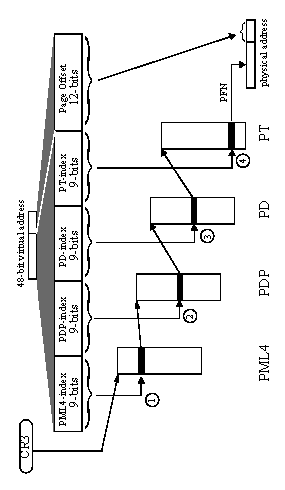
\psfig{file=FIGURES/page_table,angle=-90,width=\columnwidth}}
%	\centerline{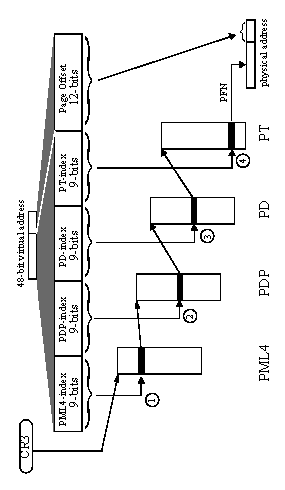
\psfig{file=FIGURES/page_table,angle=-90,width=\textwidth}}

	\caption{\small A four-level hierarchical page table.
	\normalsize}
\label{fig:page_table} 
\vspace{-0. in}
\end{figure}

% !TEX root = main.tex
% \newpage

\section{Background and Motivation} 
\label{sec:background}

\noindent Virtual memory is ubiquitous in nearly all computing systems
today and is responsible for translating virtual addresses to physical
addresses. Address translation is performed by maintaining an
application {\em page table} in system memory.
Figure~\ref{fig:page_table} shows a typical four-level hierarchical
page table commonly used in computing systems today. Each node in the
page table is 4KB in size and contains 512 8-byte entries that point
to the next node in the page table. The leaf node contains the
physical address mapping. Generally, the page table is sparsely
populated and new nodes are created only when data is referenced. As
such, the typical in-memory storage space for the application page
table is roughly 0.2\% of the total memory footprint (8 bytes of
storage overhead when using 4KB pages).

% Modern processors provide hardware support for address translation
% using the Memory Management Unit (MMU) and Input/Output MMU (IOMMU).
% The MMU handles CPU requests while the IOMMU handles device requests
% (e.g. GPU). 

Figure~\ref{fig:page_table} illustrates a {\em page walk} for a
four-level page table. The Memory Management Unit (MMU) (or page
walker) first consults a predetermined register (e.g. CR3 register on
x86 systems) to determine the physical address for Page Map Level 4
(PML4) or root node of the page table. The MMU indexes PML4 to fetch
the Page Directory Pointer (PDP) or third-level page table (first
memory reference). Next, the MMU indexes the PDP to fetch the Page
Directory (PD) or second-level page table (second memory reference).
Next, the MMU indexes the PD to fetch the first-level of the Page
Table (PT) (third memory reference). Finally, the MMU indexes the PT
(fourth memory reference) to fetch the physical address mapped to the
virtual address.

% \footnote{\noindent \small{In a virtualized environment, a
% page walk by the guest operating system may require up to 16 memory
% references}}.

% \begin{figure}[t] 
% \vspace{0. in}
% \centering
% \centerline{\psfig{file=GRAPHS/motivation_perf_mpki,angle=-90,width=\columnwidth}}
% 
% 	\caption{\small Workloads incur significant performance
% 	overhead due to frequent LLT misses. \normalsize}
% 
% \label{fig:llt_missrate} 
% \vspace{-0.15 in}
% \end{figure}

%\begin{figure}[t] 
%\vspace{0. in}
%\centering
%\centerline{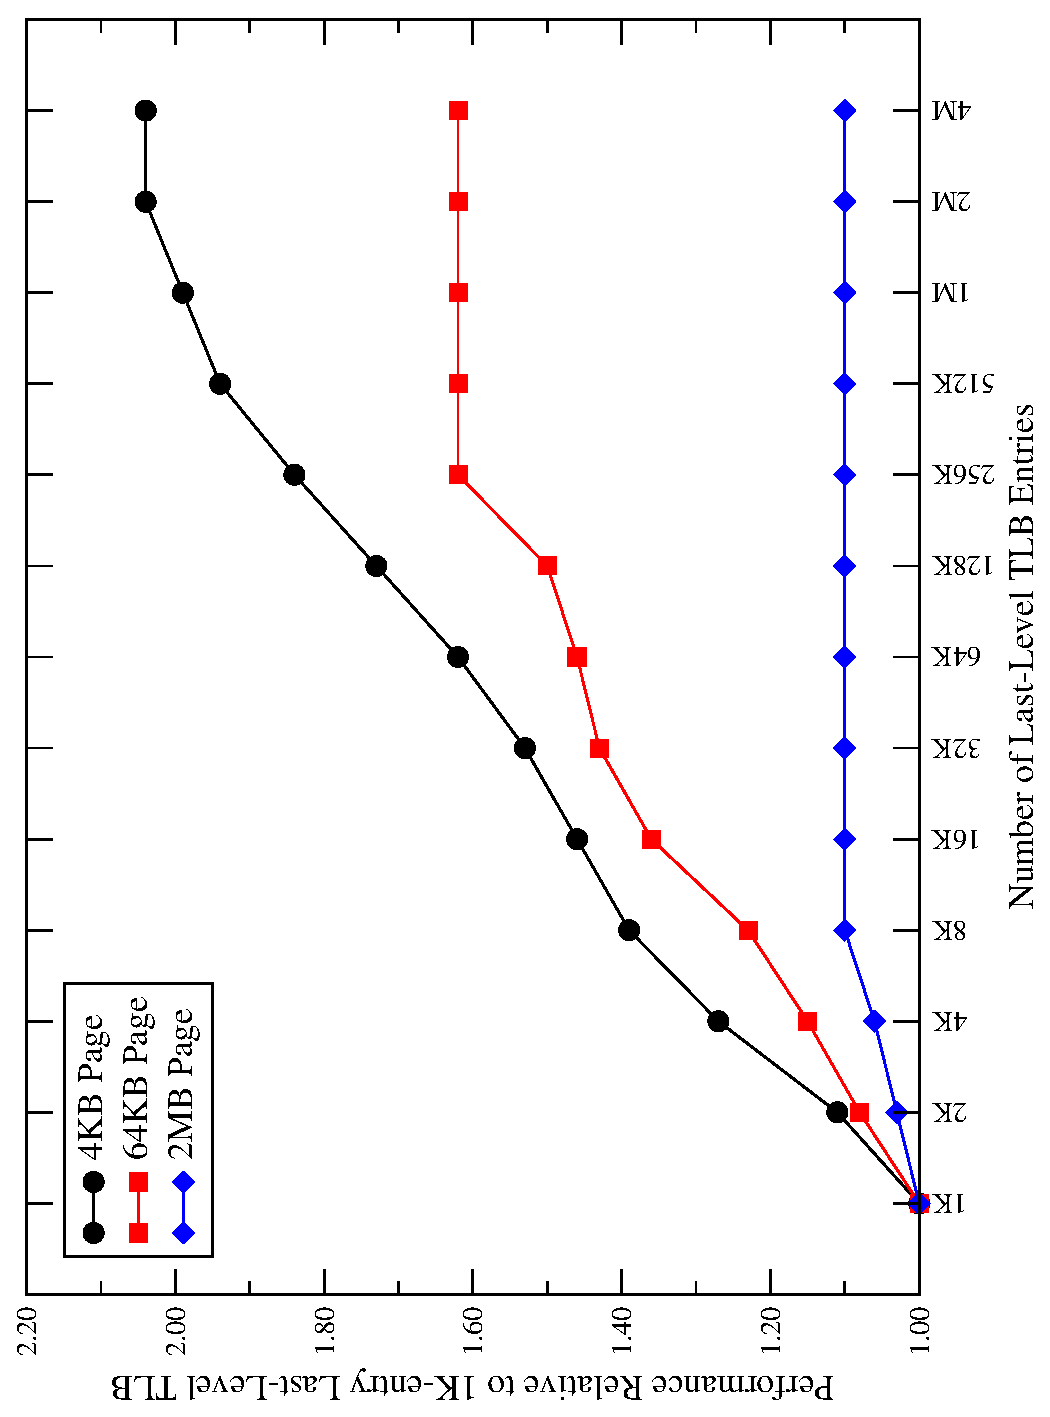
\psfig{file=GRAPHS/tlb_sensitivity,angle=-90,width=\columnwidth}}

%	\caption{\small Performance Sensitivity to LLT Entries. \normalsize}

%\label{fig:tlb_sensitivity} 
%\vspace{-0.15 in}
%\end{figure}
\begin{figure}[t]
\vspace{0. in}
\centering
\centerline{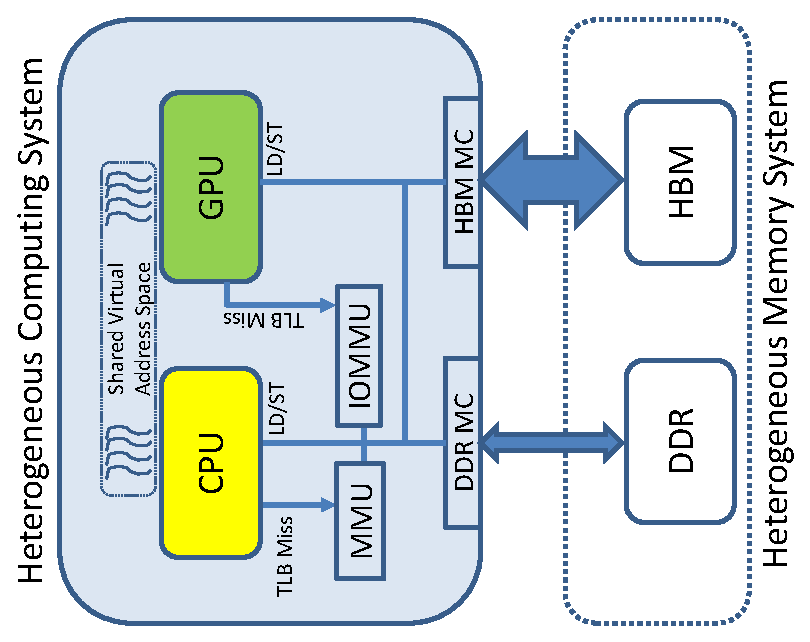
\psfig{file=FIGURES/config,scale=0.4,angle=-90}}

        \caption{\small Baseline System. \normalsize}

\label{fig:config}
\vspace{-.2 in}
\end{figure}


To reduce page table accesses on an LLT miss, commercial processors
employ Page Walk Caches (PWC) for each page table level~\cite{SkipPT,
MMUcaches}. PWCs exploit temporal and spatial locality in the page
table access stream and avoid memory accesses on PWC hits.
Consequently, the frequency of TLB misses and PWC hit rates impacts
address translation performance.

\begin {table}[b]
\small
\begin{center} 
\vspace{-0.0 in}
\caption{Workload Behavior with 4KB Page Size}
\vspace{-0. in}
\begin{tabular}{| c | c | c | c | c | }
\hline
  LLT                   & Name     &  LLT-mpki  & PT Access    &  Footprint  \\ 
  Sensitivity           &          &    & Per LLT Miss   &             \\ \hline
\multirow{5}{*}{High}   & XSBench  & 90.9       & 1.59         &  3.2 GB  \\
                        & dmr      & 81.3       & 1.81         &  1.5 GB  \\
                        & GUPS     & 92.0       & 2.00         &  15  GB  \\
                        & MaxFlow  & 86.8       & 1.83         &  1.5 GB  \\
                        & MCB      & 69.5       & 1.00         &  100 MB  \\ \hline
\multirow{6}{*}{Medium} & bfs      & 1.45       & 1.06         &  572 MB  \\
                        & LULESH   & 4.64       & 1.49         &  3.7  GB \\
                        & SNAP     & 4.81       & 1.15         &  1.6 GB  \\
                        & UMT      & 3.71       & 1.51         &  1.4 GB  \\
                        & CoMD     & 4.95       & 1.18         &  780 MB  \\
                        & HPGMG    & 6.78       & 1.54         &  4.4 GB  \\ \hline 
\multirow{3}{*}{Low}    & MiniAMR  & 5.58       & 1.62         &  3.3 GB  \\
                        & AMG      & 2.30       & 1.38         &  2.9 GB  \\ 
                        & Nekbone  & 4.36       & 1.29         &  1.1 GB  \\ \hline


\end{tabular}
\label{table:bench_char}
\vspace{-0.2in}
\end{center}
\normalsize
\end{table}


In the previous section, Figure~\ref{fig:tlb_sensitivity} motivated
increasing TLB coverage by demonstrating its direct impact on
performance. To provide further insight, Table~\ref{table:bench_char}
shows the number of LLT misses for the evaluated workloads. We observe
that these workloads incur frequent LLT misses when using 4KB pages.
To make things worse, each LLT miss requires more than one memory
access to the page table (maximum of two in some cases). Consequently,
these workloads experience significant performance overheads due to
TLB misses. With the number of levels in the page table hierarchy
expected to grow to 5-levels~\cite{x86_5level}, there is a need for
reducing the number of memory accesses on an LLT miss in addition to
improving LLT coverage. Before we describe our solutions to address
both these problems, we first provide details on our experimental
methodology.



% \begin{figure*}[tp] 
% \vspace{-0. in}
% \centering
% \centerline{\psfig{file=FIGURES/pagetable_placement,scale=0.80,angle=-90,width=\textwidth}}
% \caption{\small Different page table placement policies in a hybrid
% 	memory system. \normalsize}
% \label{fig:pagetable_placement} 
% \vspace{-0.0in}
% \end{figure*}

%\newpage
\section{Experimental Methodology}
\label{sec:method}

\noindent We assume a CPU-GPU heterogeneous system with a single CPU
and a single GPU supporting shared virtual memory~\cite{intelgen9,
amdzen} where the operating system and address translation services
are handled by the MMU and IOMMU respectively (see
Figure~\ref{fig:config}).

\begin {table}[h]
\begin{center} 
\vspace{-0.1in}
\caption{Baseline System Configuration}
\vspace{-0. in}
\begin{tabular}{|c|c|}
\hline
     \multicolumn{2}{|c|}{Streaming Multiprocessor (SM)}               \\ \hline
     Frequency            &  1 GHz                                    \\ 
     Number of SMs        &  128                                        \\ \hline
     \multicolumn{2}{|c|}{Baseline TLB and Cache Hierarchy}            \\ \hline
     L1 TLB   (private)   &  32-entry, 4-way                \\ 
     L2 TLB   (shared)    &  1024-entry, 8-way            \\ \hline
     L1 cache (private)   &  128KB,  4-way, 128B linesize  \\ 
     L2 Cache (shared)    &  8MB, 16-way, 128B linesize \\
     MSHRs for Mem Reqs   &  128 per memory channel  \\ \hline
     \multicolumn{2}{|c|}{Stacked Memory (HBM)}            \\ \hline
     Capacity             &  16GB (4 stacks)          \\
     Bus Frequency        &  1 GHz     \\ 
     Channels / Banks    &  32  / 16 per rank        \\
     Bus Width            &  128-bits per channel    \\ 
     Row Buffer Size      &  2048 Bytes              \\
     \small{tCAS-tRCD-tRP-tRAS}   &  14-14-14-33     \\ 
     Total Bandwidth      &  1024 GB/s              \\ \hline
     \multicolumn{2}{|c|}{Main Memory (DDR4)}               \\ \hline
     Capacity             &  256GB                   \\
     Bus Frequency        &  1600MHz (DDR 3.2GHz)    \\ 
     Channels / Banks    &  8  / 16 per rank        \\
     Bus Width            &  64 bits per channel     \\ 
     Row Buffer Size      &  2048 Bytes              \\
     \small{tCAS-tRCD-tRP-tRAS}   &  14-14-14-35     \\ 
     Total Bandwidth      &  204.8 GB/s               \\ \hline
     \multicolumn{2}{|c|}{Virtual Memory Configuration}     \\ \hline
%      ATS Lookup Latency   &  50 ns (oneway) \\
     Page Allocation      &  BW-aware Placement~\cite{batman,bwa}  \\ 
     Page Table (PT)      &  4-level hierarchical    \\ 
     Page Walk Caches     &  16 entries per PT level       \\ \hline

\end{tabular}
\label{table:method_system}
\vspace{-0.3in}
\end{center}
\normalsize
\end{table}


\subsection{System Configuration}

\noindent We use an industry proprietary performance simulator to
simulate a GPU (Table~\ref{table:method_system}) with memory hierarchy
based on the NVIDIA Pascal GPU system~\cite{gpu_pascal}. We model 128
Streaming Multiprocessors (SM) that support 64 warps each. A warp
scheduler selects warp instructions each cycle. The baseline GPU
memory system consists of a multii-level cache and TLB hierarchy. The
first-level cache and TLB are private to each SM while the last-level
cache (LLC) and last-level TLB (LLT) are shared by all the SMs. All
caches use 128B cache line size with 32B sectors. We assume 5 bytes of
total tag storage per LLC entry (including valid, dirty, coherence
state, and replacement bits). For the UCAT architecture, we assume an
extra 40 cycle load-to-use latency to consult the UCAT on an LLT miss.

% Each TLB supports compressing up to four contiguous TLB
% entries into a single entry~\cite{COLT}. 

We model a hybrid memory subsystem consisting of 16GB of stacked DRAM
(referred to as stacked memory) using High Bandwidth Memory (HBM)
technology~\cite{hbm-spec} and 256GB of commodity DRAM (referred to as
system memory) using conventional DDR4 technology~\cite{ddr4-spec}.
The stacked memory has 8X the bandwidth of system memory with similar
random access latency. To ensure full utilization of the total
available system bandwidth, physical pages are allocated based on the
bandwidth ratio of the hybrid memory system~\cite{bwa,batman}. In
doing so, both system memory and stacked memory satisfy memory
requests. The CPU and GPU have similar interconnect latency to the
system memory controller and stacked memory controller (50ns in both
cases). The memory controller supports 128-entry read and write queues
per channel, open-page policy, minimalist address mapping
policy~\cite{minimalist} and FR-FCFS scheduling policy (prioritizing
reads over writes). Writes are issued in batches when the write queue
starts to fill up.

% This isolates our performance studies to the bandwidth capability of
% the two memory systems rather than the latency to and from each
% individual memory system. We discuss performance implications with
% different interconnect latency (e.g. discrete CPU/GPU systems) in
% Section~\ref{sec:implications}.

We model a virtual memory system that maps virtual addresses to
physical addresses using random page replacement. Our baseline assumes
4KB page size, however we also study sensitivity to larger page size.
We model a four-level hierarchical page table~\cite{SkipPT}: Page Map
Level 4 (PML4), Page Directory Pointer (PDP), Page Directory (PD), and
Page Table (PT). All pages tables are initially allocated in low
bandwidth system memory in our baseline system. To speed up address
translation, we also model on-chip Page Walk Caches
(PWCs)~\cite{SkipPT, MMUcaches} for each page table level. The PWCs
are small, fully associative hardware structures that are indexed by
portions of the virtual address and are co-located on-chip with the
MMUs~\cite{MMUcaches}. We model a 16-entry PML4-cache, 16-entry
PDP-cache, a 16-entry PD-cache, and a 16-entry
PT-cache\cite{MMUcaches}. Finally, we assume a highly-threaded
hardware page table walker for handling misses in the
PWCs~\cite{power2014supporting, pichaigpu}.

\subsection{Workloads and Metric of Interest}

\noindent Our workloads consist of CUDA-based high performance
computing applications from the CORAL~\cite{CORAL},
Mantevo~\cite{mantevo}, and LoneStar~\cite{lonestar} suites (see
Table~\ref{table:bench_char}). The workloads are run with large inputs
to stress the hybrid memory system. We collected representative
program regions and warm up the caches, TLBs, and PWCs by
executing four billion warp instructions. After functional warmup, we
enable detailed timing simulation for two billion warp instructions.

Reduction in total execution time is our primary metric for
performance. We also compare virtual to physical address translation
latency to correlate the change in performance. We compute translation
latency as the cycles spent in translating a virtual address to
physical address averaged across all memory instructions executed by
the application.

% collect average LLT miss latency. The reduction in LLT miss latency
% directly correlates with performance improvements, we

\begin{figure*}[tp] 
\vspace{-0. in}
\centering
\centerline{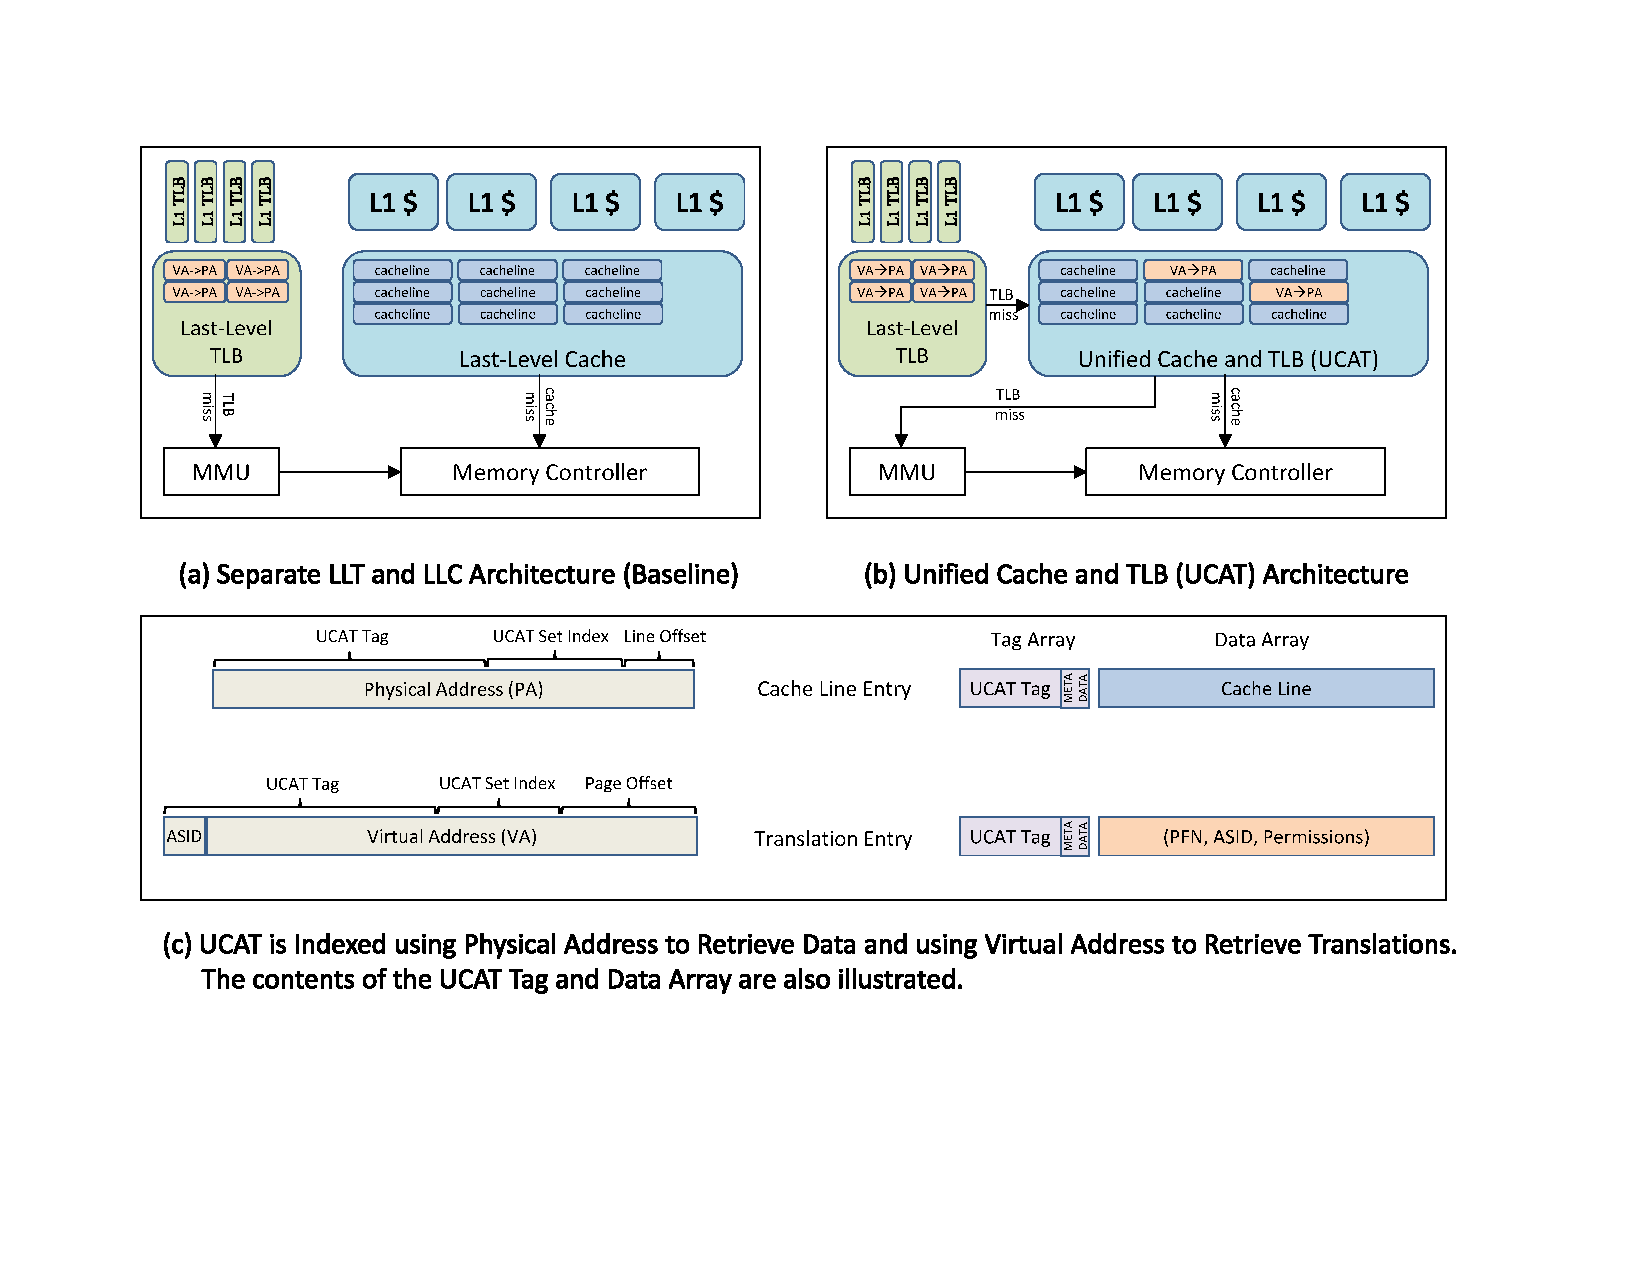
\psfig{file=FIGURES/UCAT,scale=0.80,width=\textwidth}}
\caption{\small UCAT Architecture. \normalsize}
\label{fig:pagetable_placement} 
\vspace{-0.0in}
\end{figure*}

\section{Unifying Caches and TLBs}
\label{sec:UCAT}

\noindent Modern chip multiprocessors use a multi-level TLB and cache
hierarchy to ensure high performance. The last-level in each hierarchy
is architected as a single large unified structure (holding both
instruction and data entries) that is shared across all cores. For
example, the unified last-level cache (LLC) contains several hundred
thousand cache lines\footnote{An 8MB cache with 32B lines contains
256K cache lines.}) that store data for recent memory references.
Similarly, the unified last-level TLB (LLT) contains 512-1024 TLB
entries~\cite{} that store address translations for recent memory
references.

The LLT and LLC are architected using a tag array and a data array.
The LLT tag array stores a virtual address while the LLC tag array
stores a physical memory address.\footnote{Additional meta data (e.g.
coherence state, replacement state, etc) is also stored in the tag
array.}. On the other hand, the LLT data array stores the physical
address corresponding to the virtual address translation (roughly 8
bytes) while the LLC data array stores a copy of the data from memory
at a cache line granularity (e.g. 32-64 bytes).

The LLT and LLC are cache structures with similar sized tag arrays.
Since they provide different types of data, there is a 4x-8x
difference in the data array size. We observe that, since the LLC data
array is greater than the LLT data array, the LLC can also serve as
gigantic TLB with as many entries as there are LLC lines. As such, the
conventional LLC can potentially be used to store virtual to physical
translations just like a TLB (in addition to caching data from
memory). Based on this insight, we propose to re-architect the
conventional LLC as a {\em Unified Cache and TLB (UCAT)}.

\subsection{UCAT Architecture}

\noindent A Unified Cache and TLB (UCAT) holds both cache lines and
TLB entries in a single hardware structure. Thus, a UCAT-entry is
either a cacheline or a TLB-entry. A single-bit per UCAT-entry can be
used to distinguish between the two.

In the baseline system where a UCAT-entry only stores a cache line,
the tag-array stores the physical address while the data array stores
the cache line (e.g. 32-bytes). However, when the UCAT-entry serves as
a TLB-entry, the UCAT tag-array stores the virtual address while the
data-array stores the virtual to physical address translation (roughly
8 bytes). At first, it may appear as though a large fraction of the
UCAT-entry is being wasted (e.g. 24-bytes out of a 32-byte line in our
baseline). However, recent studies have shown (and independently
verified in this study) that the majority of LLC entries are unused
after cache insertion~\cite{}. In other words, the existing LLC
entries are already inefficiently utilized. UCAT efficiently utilizes
the conventional LLC space by storing TLB entries in addition to cache
lines.

Figure X illustrates how a physical address maps to a UCAT set to
store/retrieve a cache line (baseline). Similarly we illustrate how a
virtual address maps to a UCAT set to store/retrieve a TLB entry.

% \subsection{Static UCAT Partitioning}
% 
% \noindent UCAT entries must be distributed between TLB-entries and
% cachelines. One way of accomplishing this is by statically employing
% {\em way partitioning}~\cite{}. With {\em N} ways in a UCAT set, {\em
% m} ways are statically devoted to cachelines while the remaining {\em
% N-m} ways are statically devoted to TLB entries. Cachelines are only
% inserted in the ways to devoted to them while TLB entries are inserted
% in the ways devoted to them. When evicting UCAT entries, a replacement
% policy is used (e.g. LRU, RRIP) to select between candidates within
% the same UCAT partition. We refer to this design as {\em Static UCAT
% Partitioning (UCAT-S)}.
% 
% Profiling across various workloads for different values of {\em m} can
% help arrive at the best UCAT partition for cachelines and TLB entries.
% Figure X illustrates the behavior for different {\em m}.

\begin{figure}[tp] 
  \vspace{-0.in} \centering
  \centerline{\psfig{file=GRAPHS/UCAT_perf,angle=-90,width=\columnwidth}}

  \caption{\small Performance of DRAM-TLBs. \normalsize}
  \label{fig:perf_UCAT} 
  \vspace{0.2 in}
\end{figure}

\begin{figure}[tp] 
  \vspace{0.in} \centering
  \centerline{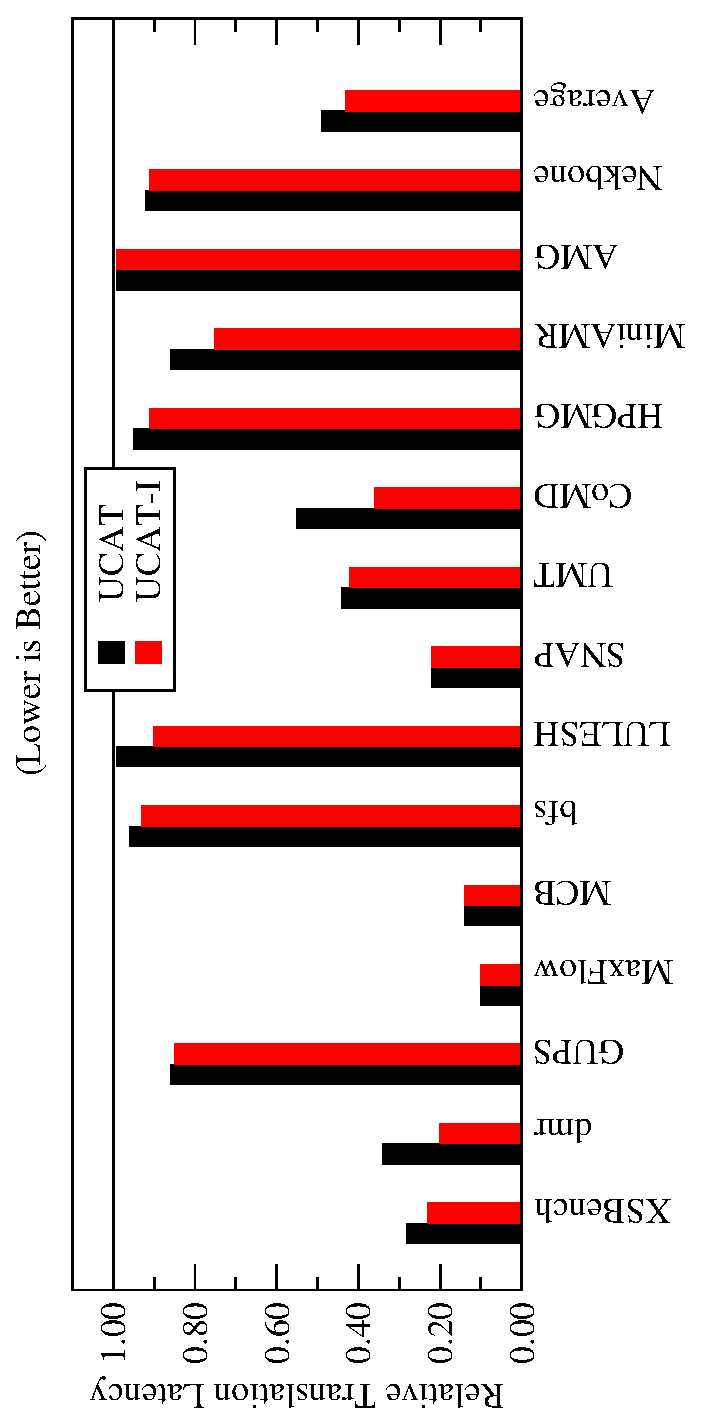
\psfig{file=GRAPHS/UCAT_tlblat,angle=-90,width=\columnwidth}}

  \caption{\small TLB miss penalty relative to baseline system.\normalsize}
  \label{fig:tlblat_UCAT} 
  \vspace{-0.1 in}
\end{figure}

\begin{figure}[tp] 
  \vspace{0.in} \centering
  \centerline{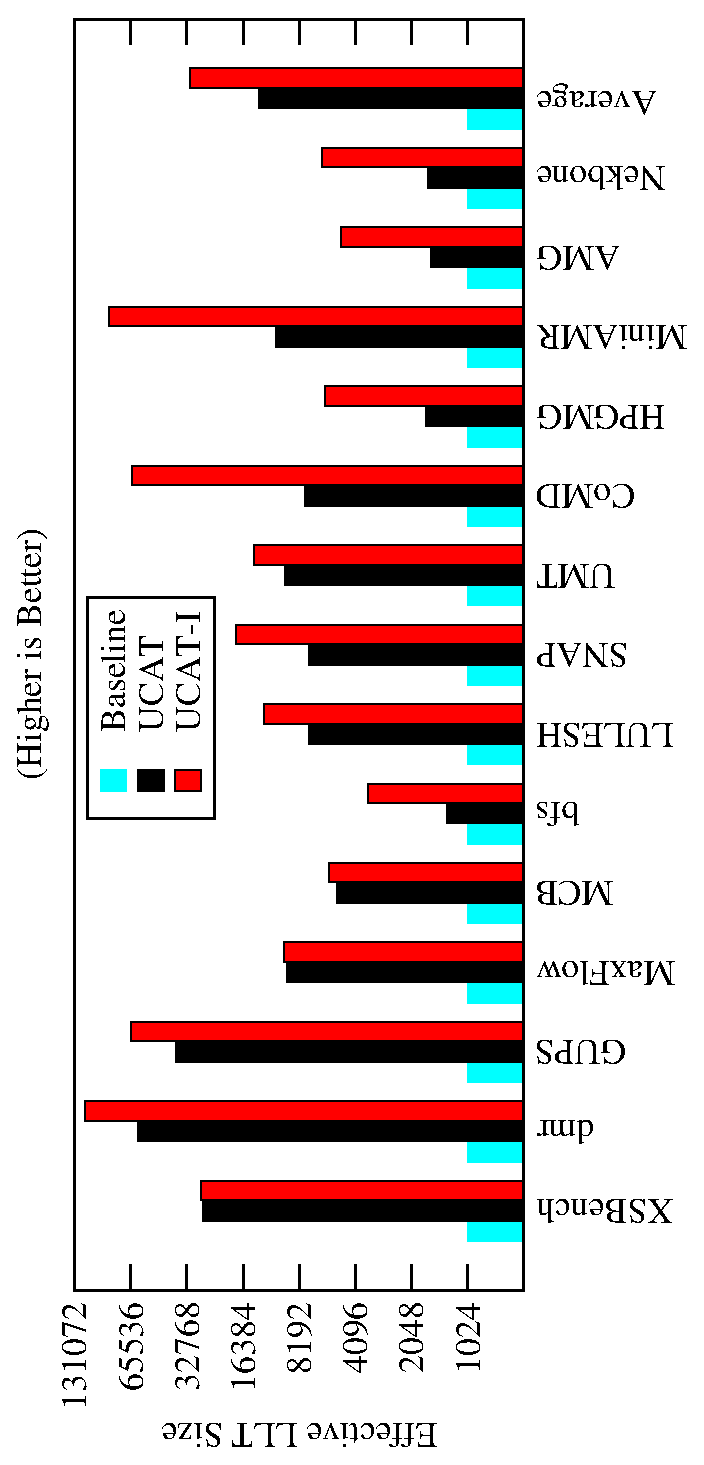
\psfig{file=GRAPHS/UCAT_tlbsize,angle=-90,width=\columnwidth}}

  \caption{\small Effective TLB Size.\normalsize}
  \label{fig:tlblat_UCAT} 
  \vspace{-0.1 in}
\end{figure}

\subsection{UCAT Allocation and Management}

% PUCAT is inefficient when the TLB-entries and cachelines have
% different capacity requirements at run time. To address this problen,
TLB-entries and cachelines dynamically share the entries in a UCAT
set. With this approach, TLB-entries and cachelines contend with one
another to occupy UCAT space. As in the baseline LLC, a single
replacement policy is used to manage UCAT entries in a set. UCAT hits
update the replacement state appropriately while UCAT misses utilize
the conventional replacement policy to select the victim candidate
within the set.

Figure Y shows UCAT performance.

The baseline polic UCAT allocates entries based on demand, rather than
utility. As such, workloads that requently stream through a large
number of cache lines can constantly discard UCAT TLB entries. Thus,
we propose to enhance DUCAT by improving the underlying replacement
policy. Our baseline system uses the Dynamic Re-Reference Interval
Prediction (DRRIP) replacement policy~\cite{}. In this baseline
policy, all UCAT insertions follow the same re-reference prediction
(i.e. insertion policy). We propose to enhance the insertion policy
for TLB entries by inserting them with a {\em near-immediate
prediction} rather than the baseline {\em far prediction}. In doing
so, TLB entries are allowed to reside in the UCAT for a longer
duration. We refer to this enhancement as {\em UCAT with Insertion
(UCAT-I)}.

Figure Y also shows performance of UCAT-I.

\begin{figure*}[t] 
  \vspace{-0. in} \centering
%  \centerline{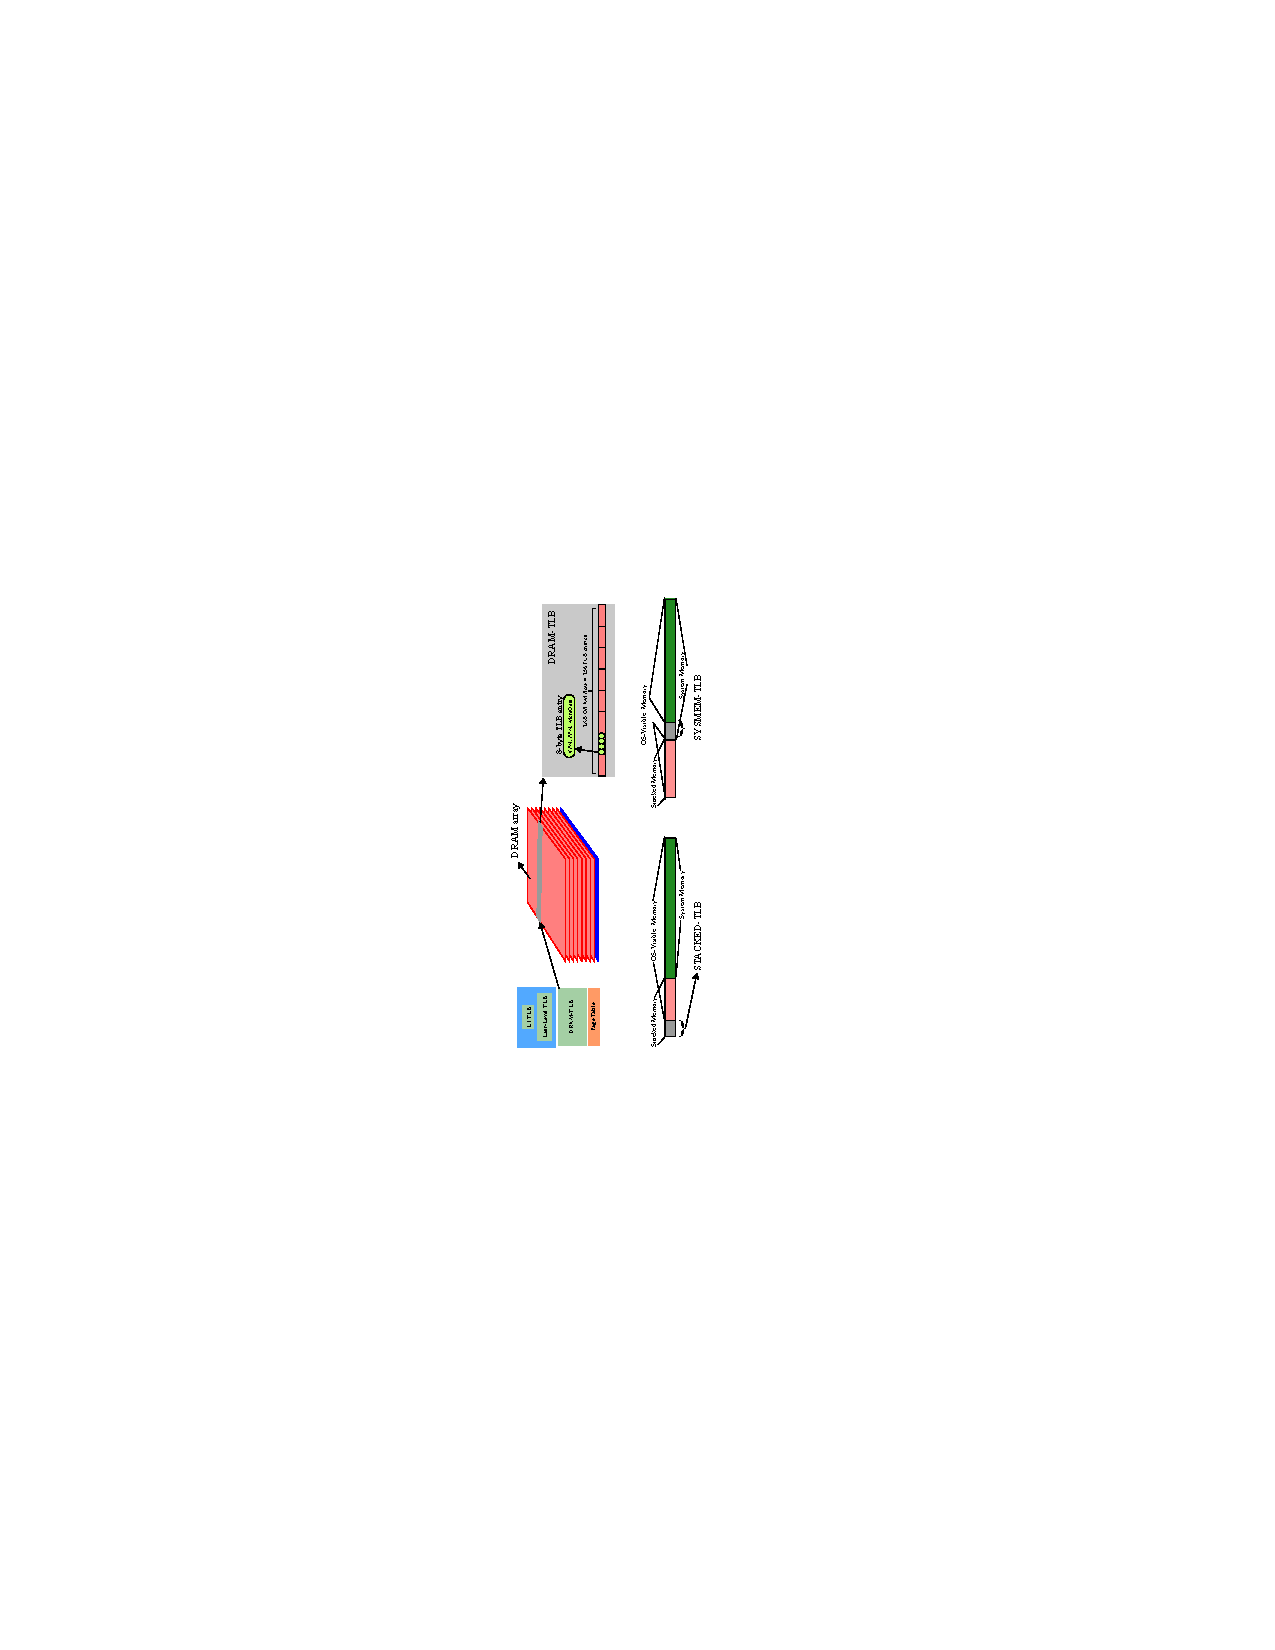
\psfig{file=FIGURES/stacked_tlb,angle=-90,width=\columnwidth}}
   \centerline{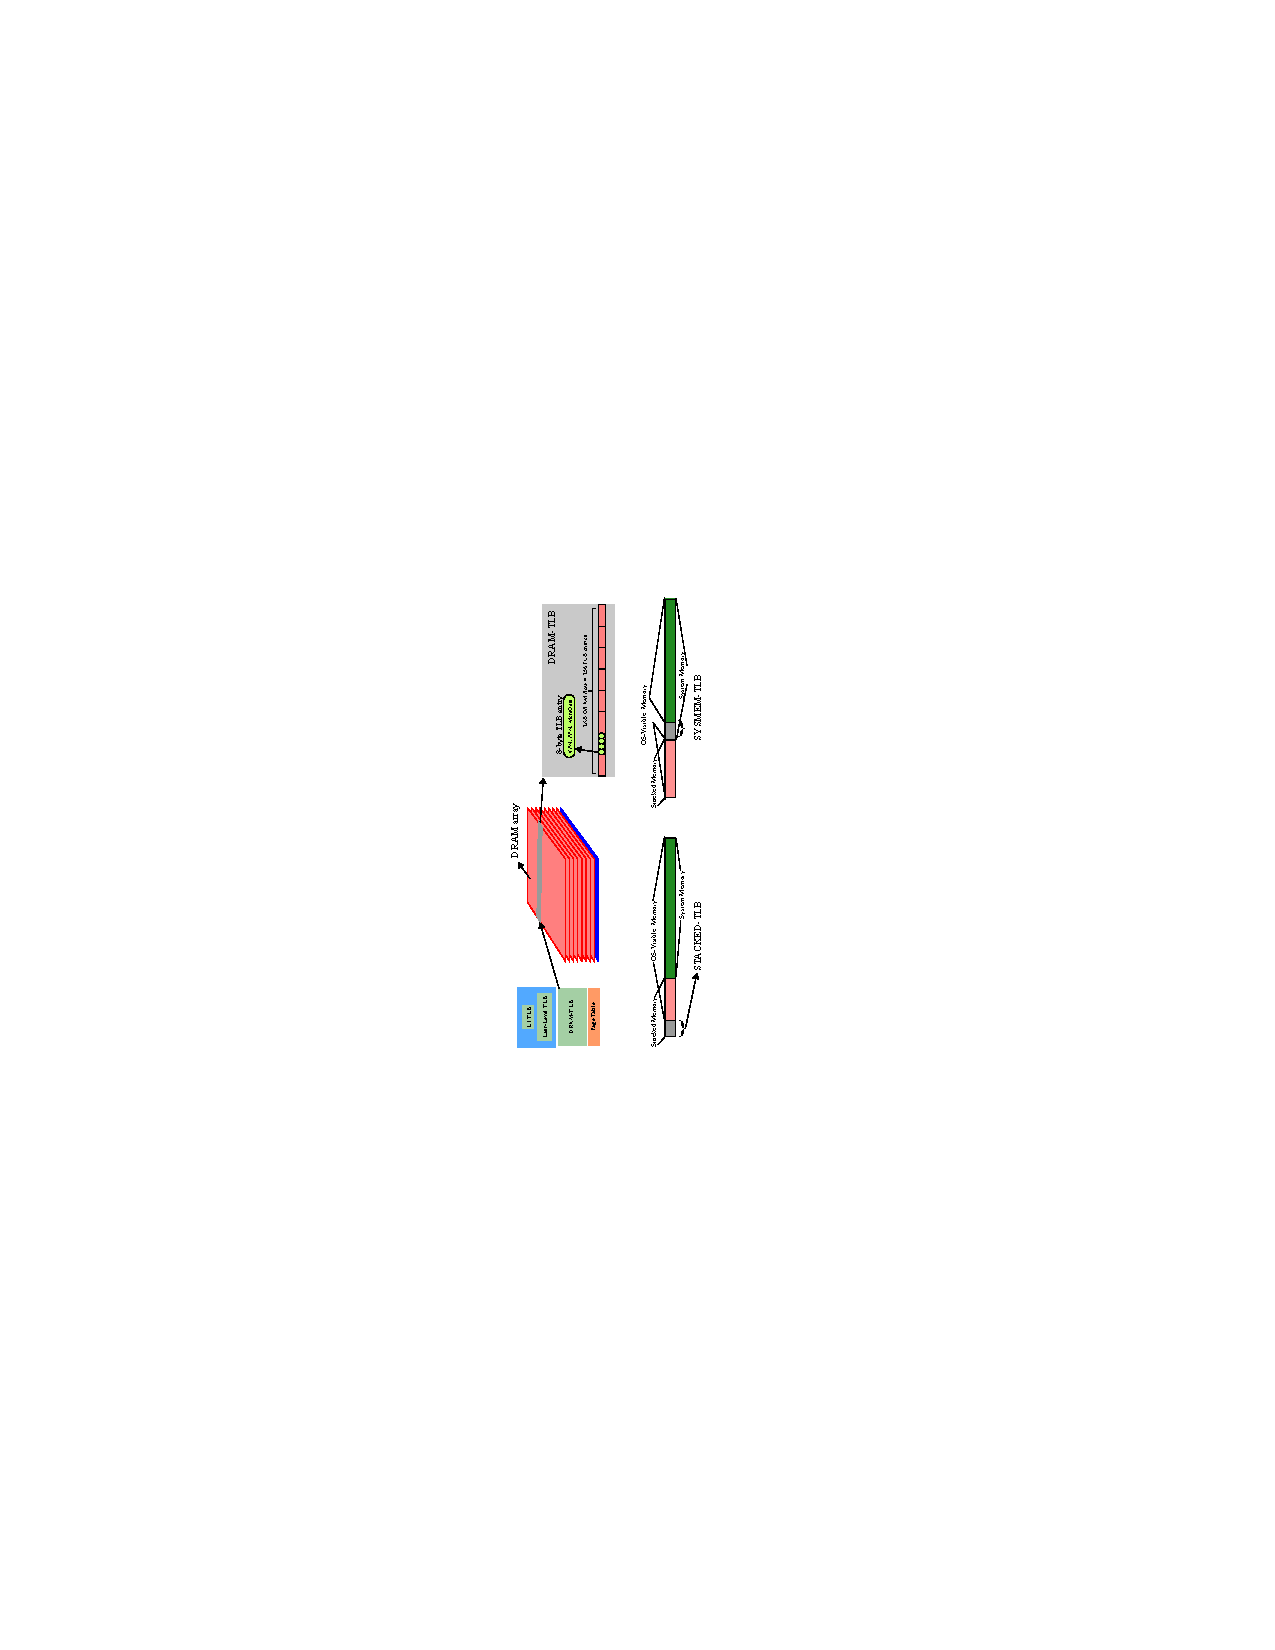
\psfig{file=FIGURES/stacked_tlb,width=\textwidth}}

  \caption{\small Improving TLB coverage by embedding TLBs in DRAM
    (DRAM-TLB). A DRAM-TLB architected using commodity DRAM is called
    SYSMEM-TLB and a DRAM-TLB architected with stacked DRAM is called
    Stacked-TLB. \normalsize}
  \label{fig:stacked_tlb} 
  \vspace{-0. in}
\end{figure*}

\subsection{UCAT Optimizations}

To avoid this additional storage overhead, we propose using the
UCAT-entry status bits (i.e. MESI bits) to make the distinction.
Specifically, we insert TLB-entries into UCAT with the {\em exclusive}
and {\em shared} status bits to be valid. Note that cachelines can
either be in exclusive state or shared state, but not both.


\section{Architecting TLBs in DRAM } 
\label{sec:stackedTLB}

\noindent When the application working set exceeds the TLB coverage
provided by UCAT (e.g. $GUPS$), UCAT does not reduce the number of
memory accesses on an LLT miss. Reducing the number of memory accesses
on an LLT miss improves memory access bandwidth and also reduces the
effective LLT miss latency.

To address this problem, we propose to increase TLB coverage and
extend the processor TLB hierarchy by architecting {\em TLBs in DRAM
(DRAM-TLB)}. The DRAM-TLB logically sits between the on-die shared LLT
(or UCAT) and the page tables in memory and is first consulted on an
LLT (or UCAT) miss before walking the page table (see
Figure~\ref{fig:stacked_tlb}).

% \noindent Recent proposals extend the processor cache hierarchy by
% architecting stacked memory as a high capacity hardware-managed DRAM
% cache~\cite{BEAR, moin2012, unison, loh2011, jaewoong2012}. Similarly,

\begin{figure*}[t] 
  \vspace{-0. in} \centering
%  \centerline{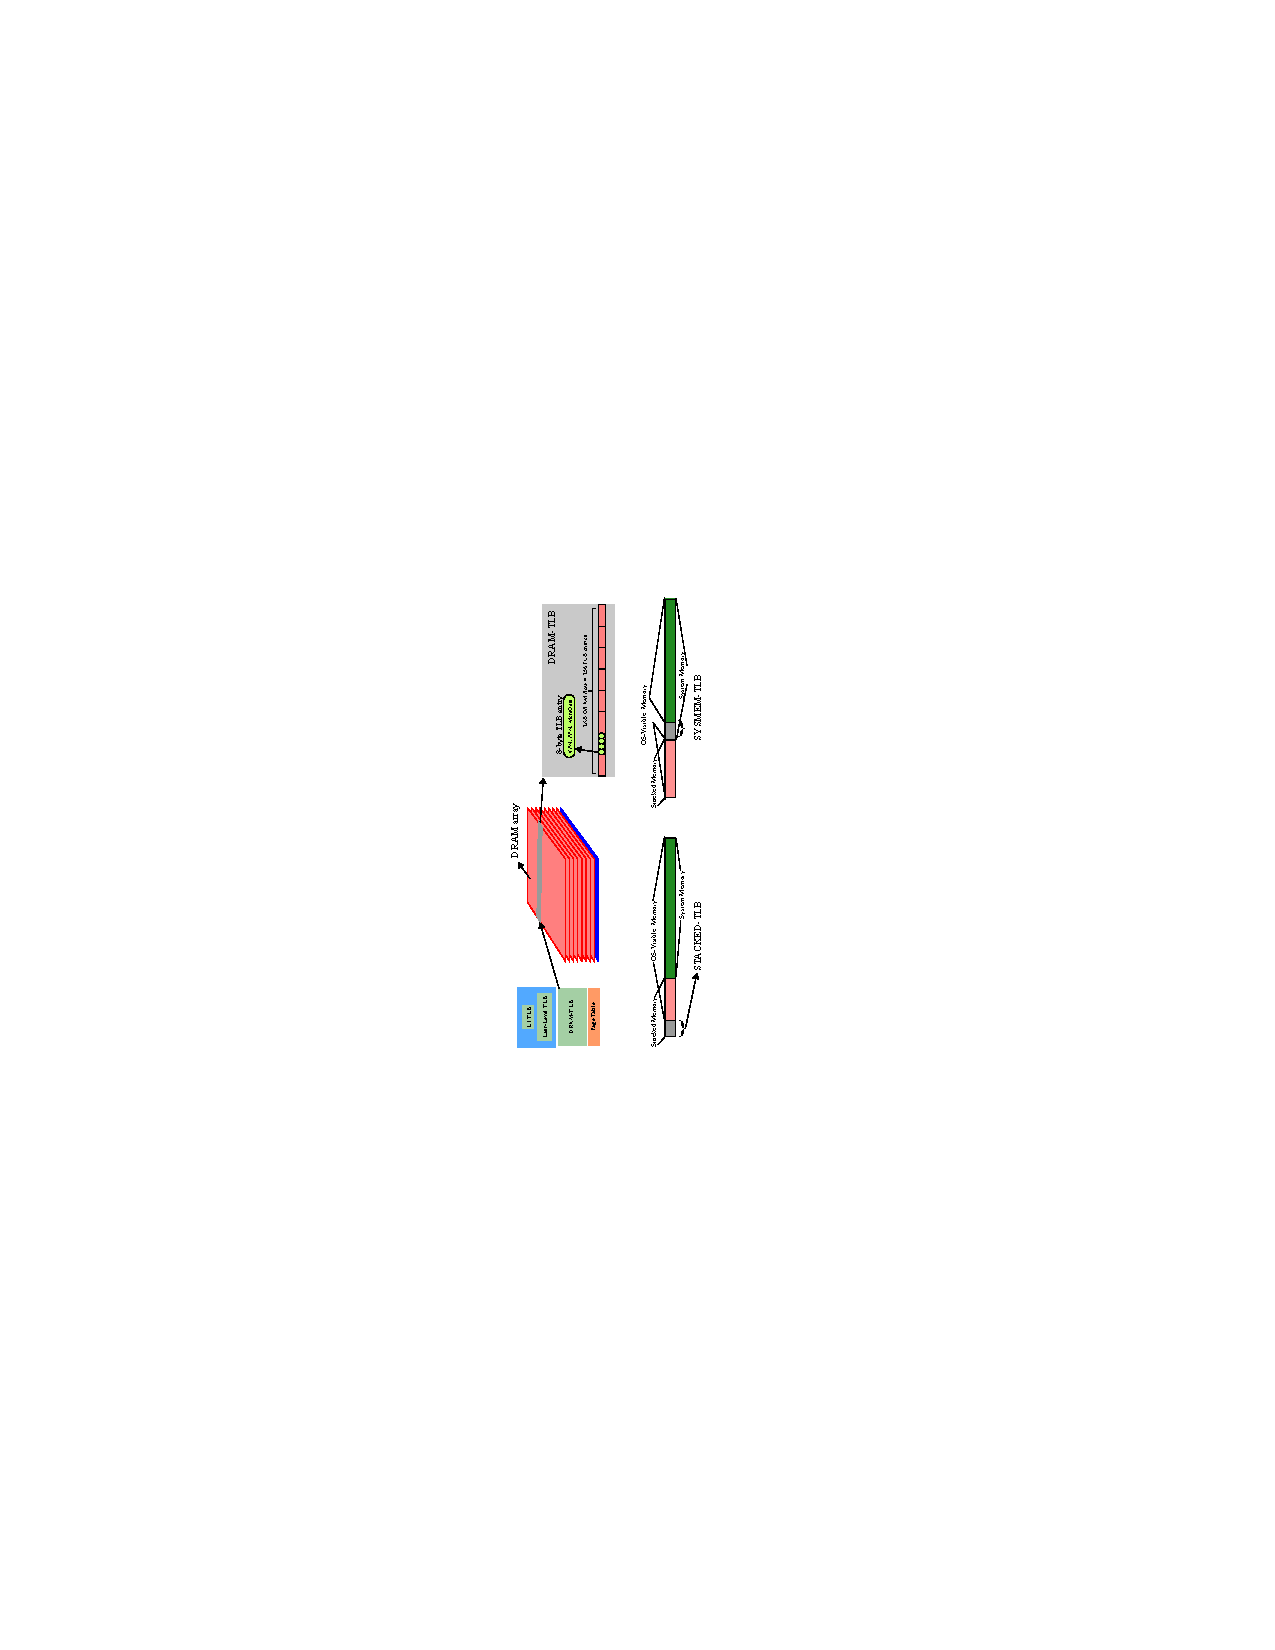
\psfig{file=FIGURES/stacked_tlb,angle=-90,width=\columnwidth}}
   \centerline{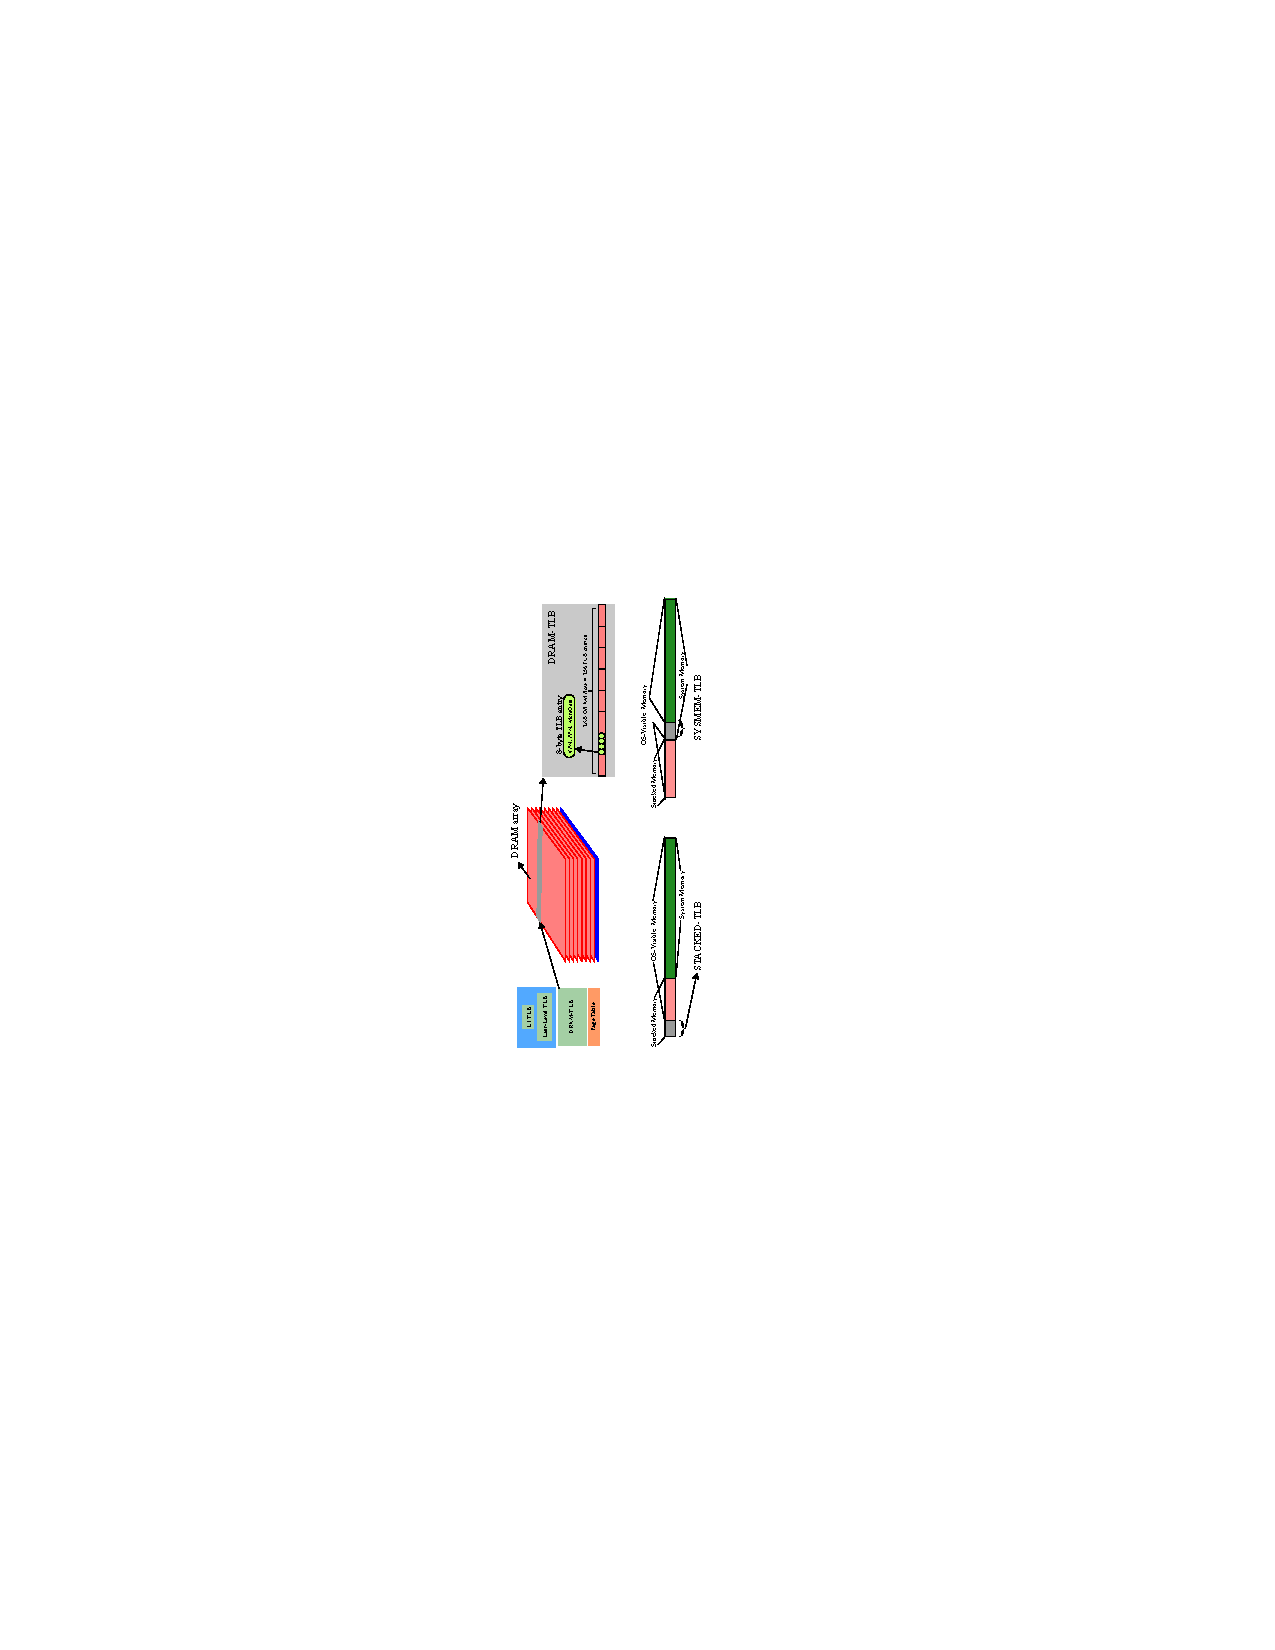
\psfig{file=FIGURES/stacked_tlb,width=\textwidth}}

  \caption{\small Improving TLB coverage by embedding TLBs in DRAM
    (DRAM-TLB). A DRAM-TLB architected using commodity DRAM is called
    SYSMEM-TLB and a DRAM-TLB architected with stacked DRAM is called
    Stacked-TLB. \normalsize}
  \label{fig:stacked_tlb} 
  \vspace{-0. in}
\end{figure*}

\subsection{DRAM-TLB Architecture}

\noindent DRAM-TLBs can either be architected using stacked memory or
system memory. A DRAM-TLB architected using stacked memory is referred
to as a {\em Stacked-TLB} while a DRAM-TLB architected using system
memory is referred to as a {\em SYSMEM-TLB}. DRAM-TLBs are physically
placed in a large contiguous segment of memory and are entirely
hardware-managed. As such, DRAM-TLBs do not contribute to the
OS-visible memory space (see Figure~\ref{fig:stacked_tlb}(c)).

% illustrates, DRAM-TLBs and the OS-visible
% address space when the hybrid memory system is configured with a
% SYSMEM-TLB or a Stacked-TLB.

\subsubsection{DRAM-TLB Organization}

\noindent Like conventional on-chip SRAM TLBs, and the proposed UCAT
architecture, a DRAM-TLB entry maintains the TLB tag, physical
address, and meta data information such as valid bits, page permission
bits, address space identifier (ASID), and the epoch counter (EPCTR).
To accommodate this information, we propose 16 bytes of storage per
DRAM-TLB entry. Figure~\ref{fig:stacked_tlb} illustrates the layout of
the DRAM-TLB in the DRAM array. For example, a 2KB DRAM array holds
128 DRAM-TLB entries per rowbuffer.

\subsubsection{DRAM-TLB Lookups}

\noindent Unlike on-chip TLBs, all DRAM-TLB operations occur on the
DRAM data bus at the granularity of the DRAM read/write interface.
Thus, on an LLT miss, a Stacked-TLB lookup fetches data at the
granularity of the stacked memory interface: 32-byte cacheline (two
TLB entries). While SYSMEM-TLB lookup fetches data at the granularity
of the DDR interface: 64-byte cacheline (four TLB entries).

Reading multiple TLB entries with a single DRAM read operation can be
exploited in two ways. First, retrieving the co-located DRAM-TLB
entries on a DRAM-TLB read naturally enables prefetching of
neighboring address translations. For example, prefetched entries can
potentially be stored in an on-chip TLB prefetch buffer. This approach
is similar to caching co-located page table entries in the page walk
cache on a conventional page table walk. Alternately, reading multiple
TLB entries enables architecting a set-associative DRAM-TLB without
incurring additional latency or bandwidth~\cite{moin2012,loh2011}. 

We explored the design space of set-associative and direct-mapped
DRAM-TLBs. Our studies with both set-associative and direct-mapped
designs yielded similar performance with large DRAM-TLB sizes. These
results match the behavior of existing work on large DRAM Caches where
conflict misses tend to be low~\cite{moin2012}. Thus, we architect a
direct-mapped DRAM-TLB where consecutive DRAM-TLB sets map to the same
rowbuffer in memory (to exploit DRAM row buffer locality). Adjacent
DRAM-TLB entries fetched are also inserted into the PWC for potential
future hits.

% Similar to page walk caches, we also provision an 8-entry
% DRAM-TLB-Cache (DTLBcache) that stores recent lines retrieved from the
% DRAM-TLB. In doing so, the DTLBcache exploits spatial locality in LLT
% misses.

\subsubsection{DRAM-TLB Insertions and Updates}

\noindent The DRAM-TLB must be updated on misses, shootdowns, and page
permission changes. We propose to modify the TLB-entry directly in
DRAM on updates. To ensure that updating a single DRAM-TLB-entry does
not corrupt the contents of co-located DRAM-TLB entries, we leverage
existing DRAM interfaces that allow partial writes (e.g. byte-level
writes) to memory without the power and bandwidth overhead of a full
read-modify-write operation~\cite{hbm-spec}.


% If the DRAM-TLB entry exists in the DTLBcache, the corresponding entry
% is directly updated in the DTLBcache. However, if the entry does not
% exist in the DTLBcache,




% \begin{figure}[htb] 
% \vspace{-0. in}
% \centering
% 	\centerline{\psfig{file=GRAPHS/stackedDRAMTLB_cachelat,angle=-90,width=\columnwidth}}
% 
% \caption{\small This figure compares the average LLC miss latency of
% 	DRAM-TLB and Stacked-TLB relative to the baseline system. \normalsize}
% \label{fig:cachelat_DRAMTLB} 
% \vspace{-0. in}
% \end{figure}

\subsubsection{DRAM-TLB Implementation}

% If the request can be serviced from the first-level page table, the
% MMU follows the baseline address translation policy and fetches the
% translation from the first-level page table. This is because
% retreiving the first-level page table entry and a DRAM-TLB lookup both
% require a single memory access.

% If the MMU is required to access more than one level of the page
% table, we propose that the

\noindent Since the DRAM-TLB is located in physical memory, the
physical location of the DRAM-TLB entry must first be determined. We
propose an 8-byte register in the Memory Management Unit (MMU) to
store the base address $BaseAddr$ for the DRAM-TLB. Given the DRAM-TLB
set index {\em SI} of the missing virtual address, DRAM-TLB
associativity $A$, and DRAM-TLB entry size $s$ (16 bytes in our case),
the DRAM-TLB entry physical address is computed using combinational
logic:

\begin{equation}
  \begin{array}{rl}
    \text{PhysAddr} = BaseAddr + SI * A * s
  \end{array}
\end{equation}

\noindent Once the DRAM-TLB entry is retrieved from memory, a tag
comparison is performed to determine hit or miss. On a DRAM-TLB hit,
the missing translation is returned to the processor. However, on a
DRAM-TLB miss, the application page table is walked to find the
virtual to physical translation. This translation is returned to the
processor and also inserted into the DRAM-TLB for future hits.

\subsubsection{DRAM-TLB Example}

\noindent Assume a 1M-entry direct-mapped DRAM-TLB (with 4KB pages)
starting at memory location {\em BaseAddr=0}. An LLT miss for virtual
page 0xff2212345000 requires fetching the 16-byte DRAM-TLB entry at
set index 0x12345. With $A=1$ and $s=16$, the physical memory location
for this DRAM-TLB entry is 0x123450 (i.e. 0 + 0x12345 * 1 * 16). The
MMU compares the missing tag (0xff22) with the DRAM-TLB entry to
determine DRAM-TLB hit or miss.

\subsection{DRAM-TLB Performance}

% For our evaluation purposes, we do not exploit the prefetching
% benefits from fetching multiple TLB entries with a single DRAM read
% operation.

% \subsubsection{Steady State Performance Behavior}

% Since our application
% have memory footprint less than 32GB, both DRAM-TLB configurations
% incur only compulsory misses and behave like a {\em perfect} DRAM-TLB
% in steady state.

% illustrates the workloads on the x-axis and the performance relative
% to our baseline system on the y-axis. The figure

\noindent We evaluate SYSMEM-TLB and Stacked-TLB performance assuming
an 8-million entry DRAM TLB (32GB TLB coverage with 4KB pages).
Figure~\ref{fig:perf_DRAMTLB} shows that DRAM-TLBs improve performance
relative to the baseline system across all TLB-sensitive workloads. On
average, SYSMEM-TLB improves performance by 11\% while Stacked-TLB
improves performance by 22\%. In general, Stacked-TLBs perform better
than SYSMEM-TLBs because they are architected with stacked memory, a
technology that provides high memory bandwidth and less memory queing
delays. As illusrated in Figure~\ref{fig:tlblat_DRAMTLB}, unlike
SYSMEM-TLBs that reduce address translation latency by 12\% on
average, Stacked-TLBs reduce address translation latency by 40\% on
average. The translation latency reduction stems from the fact that
DRAM-TLBs reduce the number of memory accesses on an LLT miss from 1.6
memory accesses to a single memory access on average (see
Figure~\ref{fig:memaccess_DRAMTLB}). The improved translation latency
boosts performance of workloads like $GUPS$ and $MaxFlow$ by more than
70\%. On the other hand, workloads like $XSBench$, $dmr$, $LULESH$ and
$MiniAMR$ experience more than 15\% performance gain.

% % \subsubsection{Non-Steady State Performance Behavior}
% % 
% % \noindent Under steady state conditions, SYSMEM-TLBs are competitive
% % with Stacked-TLB despite being architected using low bandwidth
% % commodity DRAM. However, in practice workloads tend to go through
% % phases of execution where misses occur in the DRAM-TLB. As such, we
% % now study how SYSMEM-TLBs and Stacked-TLBs behave when they experience
% % TLB misses.
% % 
% % \begin{figure}[t] 
% %   \vspace{-0. in}
% %   \centering
% %   \centerline{\psfig{file=GRAPHS/stackedDRAMTLB_hitrate_sens,angle=-90,width=\columnwidth}}
% % 
% %   \caption{\small Sensitivity to DRAM-TLB hit-rate. \normalsize}
% % 
% %   \label{fig:hitrate_DRAMTLB} 
% %   \vspace{-0. in}
% % \end{figure}
% % 
% % The overhead of a DRAM-TLB miss is the wasted bandwidth to consult the
% % DRAM-TLB and the bandwidth to insert the missing entry into the
% % DRAM-TLB. In general, these operations consume precious DRAM
% % bandwidth. When bandwidth is scarce, both these operations can degrade
% % performance significantly since they do not contribute towards useful
% % work. To understand this phenomenon,
% % Figure~\ref{fig:hitrate_DRAMTLB} illustrates the performance
% % behavior of SYSMEM-TLBs and Stacked-TLBs as a function of
% % hit-rate\footnote{A statistical model that samples a random number
% % generator is used to achieve the desired DRAM-TLB hit rate.}. The
% % x-axis shows the TLB hit rate while the y-axis shows the performance
% % relative to the baseline system averaged across all workloads.
% % 
% % In steady state (i.e. when the TLB hit rate is a 100\%) both
% % Stacked-TLB and SYSMEM-TLB perform well. However, when the hit-rate
% % reduces, DRAM-TLB lookup and DRAM-TLB fill operations start consuming
% % precious DRAM bandwidth. This additional bandwidth quickly degrades
% % SYSMEM-TLB performance. For example, at 80\% hit rate, SYSMEM-TLB
% % performance plunges from 38\% performance improvement to a mere 8\%
% % performance improvement. Continuing to follow the hit-rate curve,
% % SYSMEM-TLBs degrade performance at DRAM-TLB hit-rates below 70\%.
% % These results show that SYSMEM-TLBs are useful only if they can
% % provide near-optimal hit-rate. Unfortunately ensuring a 100\% hit-rate
% % is impossible without future knowledge.
% % 
% % Stacked-TLBs are less sensitive to degradation in hit-rate. An 80\%
% % Stacked-TLB hit-rate retains performance improvement (34\% vs 42\%).
% % Following the hit-rate curve, Stacked-TLBs degrade performance only
% % when the hit-rate drops below 30\% (which is unlikely). Consequently,
% % this suggests that Stacked-TLBs are more suitable alternative to
% % SYSMEM-TLBs. Hereon, we only report performance results for
% % Stacked-TLBs.

% <------------GRAVEYARD
% Both DRAM-TLB and Stacked-TLB improve performance because they reduce
% the address translation bandwidth and address translation latency. In
% doing so, the LLT miss latency reduces by (see ).

% Furthermore, since Stacked-TLBs handle changes in hit-rate gracefully,
% we report performance results for workloads in steady state.

% This suggests that the bandwidth capability of stacked memory enables
% Stacked-TLBs as a viable hardware structure to increase the TLB
% hierarchy.

% Unfortunately, the first order performance bottleneck of DRAM-TLB
% misses is bandwidth. If the DRAM-TLB lookup misses, that is wasted
% bandwidth. Inserting a missing translation into the DRAM-TLB requires
% bandwidth.

% Consequently such requests consume precious system memory bandwidth.
% Furthermore, to DRAM-TLBs

% If DRAM-TLBs can constantly provide hits, they reduce the 1.75 memory
% accesses per LLT miss our workloads observe to a single memory access.
% However, DRAM-TLBs can suffer from misses too. Especially when the
% application footprint exceeds the coverage of the DRAM-TLB. This
% problem can be addressed by simply sizing the DRAM-TLB to cover the
% largest possible application memory footprint. In our experience, the
% majority of DRAM-TLB misses are compulsory misses. Once the workload
% reaches steady state, a DRAM-TLB effectively behaves like a {\em
% perfect} TLB.

% If the workloads frequently miss in the DRAM-TLB, both the latency and
% required bandwidth for address translation increases. This is because
% a DRAM-TLB miss incurs two additional memory accesses: one for missing
% in the DRAM-TLB and the other for inserting the missing DRAM-TLB.


% Note, however that the DRAM-TLB lookup is on the critical path while
% the DRAM-TLB fill can be done in the background. Thus, the memory
% bandwidth penalty of a DRAM-TLB miss is two requests, but the latency
% penalty is one memory access.

% Therefore, the total cost
% of a DRAM-TLB miss is the cost of one memory access serialization latency plus
% any queuing delays due to the DRAM-TLB fill.

% To quantify the desired behavior of DRAM-TLBs, both from miss traffic
% and miss latency perspective, 

% Figure~\ref{fig:hitrate_DRAMTLB} illustrates the required
% DRAM-TLB hit rate to equalize the average address translation traffic
% and the average address translation latency (assuming DRAM-TLB fills
% do not significantly impact memory access latency) respectively. The
% x-axis illustrates the average number of page table memory accesses
% per LLT miss while the y-axis illustrates the required DRAM-TLB hit
% rate.

% Clearly, if the average number of page table accesses per LLT miss is
% one, we would require a 100\% DRAM-TLB hit rate. As described earlier
% in the paper, this would normally occur when the MMU always hits in
% the second-level page table cache. In such situations, the MMU can
% just bypass the DRAM-TLB lookup altogether and just fetch the
% translations directly from the page table.
% 
% However, the majority of our applications require more than one page
% table access per LLT miss (ranging between 1.40 and 2.25). These page
% table access rates require a DRAM-TLB hit-rate ranging between 40\%
% and 80\%. Achieving these hit rates is well within the range of
% DRAM-TLBs because their relative storage overhead is negligible.
% However, in pathological situations where the DRAM-TLB hit-rate is
% well below the desired break-even hit rate (e.g. streaming workload),
% the MMU can dynamically bypass the DRAM-TLB state machine altogether.


% \begin{figure}[t] 
% \vspace{-0. in}
% \centering
% 	\centerline{\psfig{file=GRAPHS/stackedDRAMTLB_break_even,angle=-90,width=\columnwidth}}
% 
% \caption{\small This figure illustrates a sensitivity study for the
%   required DRAM-TLB hit rate for different pagetable requests per LLT miss. \normalsize}
% \label{fig:hitrate_DRAMTLB} 
% \vspace{-0. in}
% \end{figure}
%------------------> GRAVEYARD

\begin{figure}[tp] 
  \vspace{-0.in} \centering
  \centerline{\psfig{file=GRAPHS/DRAMTLB_perf,angle=-90,width=\columnwidth}}

  \caption{\small Performance of DRAM-TLBs. \normalsize}
  \label{fig:perf_DRAMTLB} 
  \vspace{0.2 in}
\end{figure}

\begin{figure}[tp] 
  \vspace{0.in} \centering
  \centerline{\psfig{file=GRAPHS/DRAMTLB_tlblat,angle=-90,width=\columnwidth}}

  \caption{\small Translation Latency Relative to baseline.\normalsize}
  \label{fig:tlblat_DRAMTLB} 
%  \vspace{0.2 in}
\end{figure}

\begin{figure}[tp] 
  \vspace{0.in} \centering
  \centerline{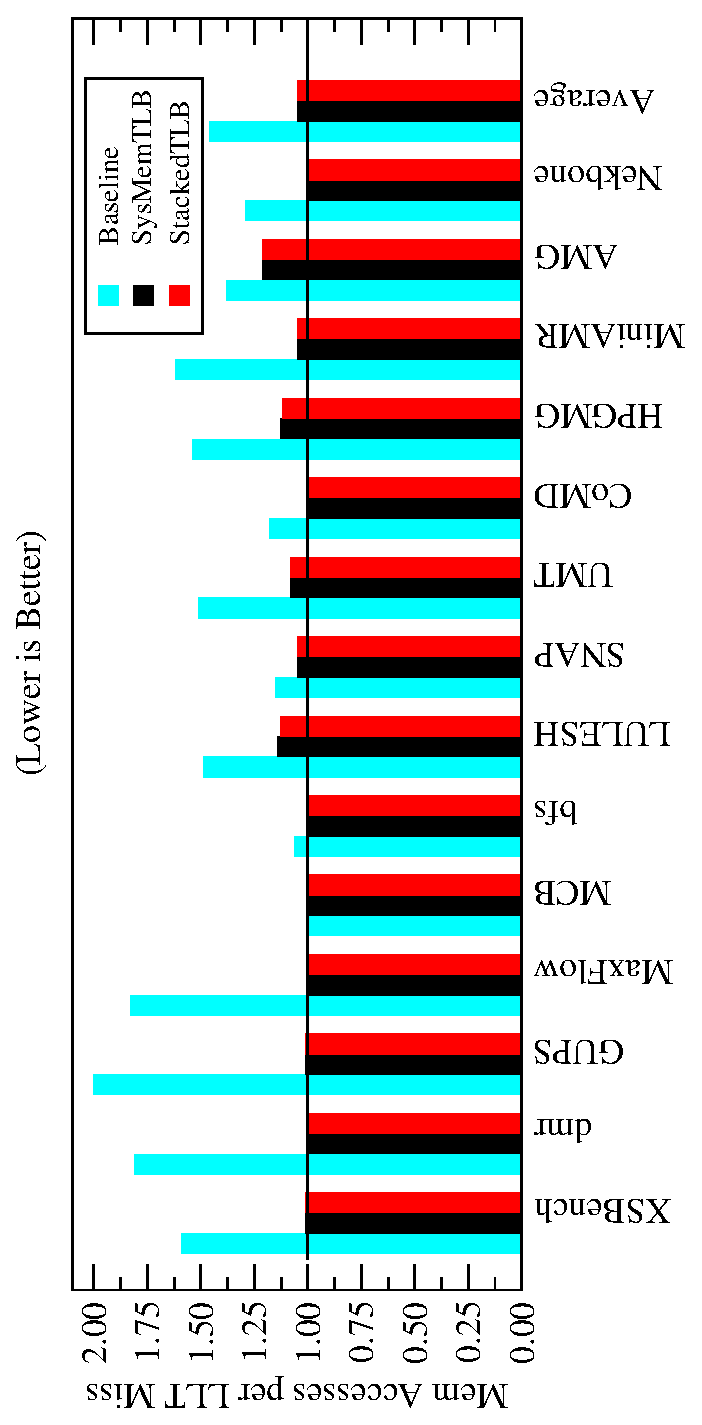
\psfig{file=GRAPHS/DRAMTLB_pteaccess,angle=-90,width=\columnwidth}}

  \caption{\small Memory Accesses on an LLT miss.\normalsize}
 \label{fig:memaccess_DRAMTLB} 
%  \vspace{-0.1 in}
\end{figure}


\subsection{DRAM-TLB Design Overhead}

\noindent We propose simple modifications to the Memory Management
Unit (MMU) state machine to support DRAM-TLBs (see
Figure~\ref{fig:mmu_state}). On an LLT miss, the MMU first consults
the page walk caches to retrieve the translation. If the request
misses in the PWCs, the MMU consults the DRAM-TLB. If the request
misses in the DRAM-TLB, the MMU walks the page table. Thus, we simply
introduce a new state in the MMU state machine for the DRAM-TLB lookup
before walking the page table.

The in-memory storage overhead for DRAM-TLBs depends on the desired
TLB coverage. For example, achieving full system memory (256GB in our
baseline) coverage with 4KB, 64KB, and 2MB pages 1GB, 64MB, and 2MB of
storage overhead (assuming 16-byte DRAM-TLB entries). In general, this
storage overhead is impractical for on-chip SRAM TLBs. However, these
sizes are an insignificant fraction of emerging multi-gigabyte stacked
memory systems. For example, the aforementioned storage overheads
correspond to 6\% (4KB pages), 0.4\% (64KB pages), and 0.01\% (2MB
pages) storage overhead for a 16GB stacked memory system.
Consequently, DRAM-TLBs can improve TLB coverage using small pages
with minimal storage overhead and most importantly require no
significant changes to the existing address translation mechanisms.

\begin{figure}[b] 
  \vspace{-0. in} \centering
  \centerline{\psfig{file=FIGURES/mmu_state,angle=-90,width=\columnwidth}}

  \caption{\small MMU extensions to support DRAM-TLBs.
    \normalsize}
  \label{fig:mmu_state} 
  \vspace{-0 in}
\end{figure}



% \subsection{DRAM-TLB Summary}
% 
% \noindent DRAM-TLB is a flexible, scalable, and low overhead mechanism
% that can provide arbitrary TLB coverage. DRAM-TLB serves as the next
% shared level in the on-chip TLB hierarchy and can reduce memory
% bandwidth requirements for address translation to a single memory
% access and can improve performance by 50\% on average (up to 2X).

% DRAM-TLBs provide an opportunity to increase the coverage of existing
% on-chip TLB hierarchies. Since, DRAM-TLBs can potentially provide
% address translations using in a single memory access, they provide an
% alternative low latency, low bandwidth solution to walking the page
% table on an LLT miss.



\section{DUCATI: Combining DRAM-TLBs \newline and UCAT}
\label{sec:DUCATI}

\noindent UCAT and DRAM-TLB independently improve on-die processor TLB
coverage and LLT miss overhead respectively. These mechanisms can be
combined to collectively improve processor performance. To this end,
we propose {\em DUCATI}, an address translation architecture that
combines \underline{D}RAM-TLBs and \underline{UCAT-I}. While DUCATI
can be architected with Stacked-TLBs or with SYSMEM-TLBs, we limit our
analysis of DUCATI to Stacked-TLBs. This is because stacked memory
technology provides better bandwidth and latency than with
conventional DDR memory technology.

\subsection{DUCATI Performance}

\begin{figure}[tp] 
\vspace{-0 in} \centering
\centerline{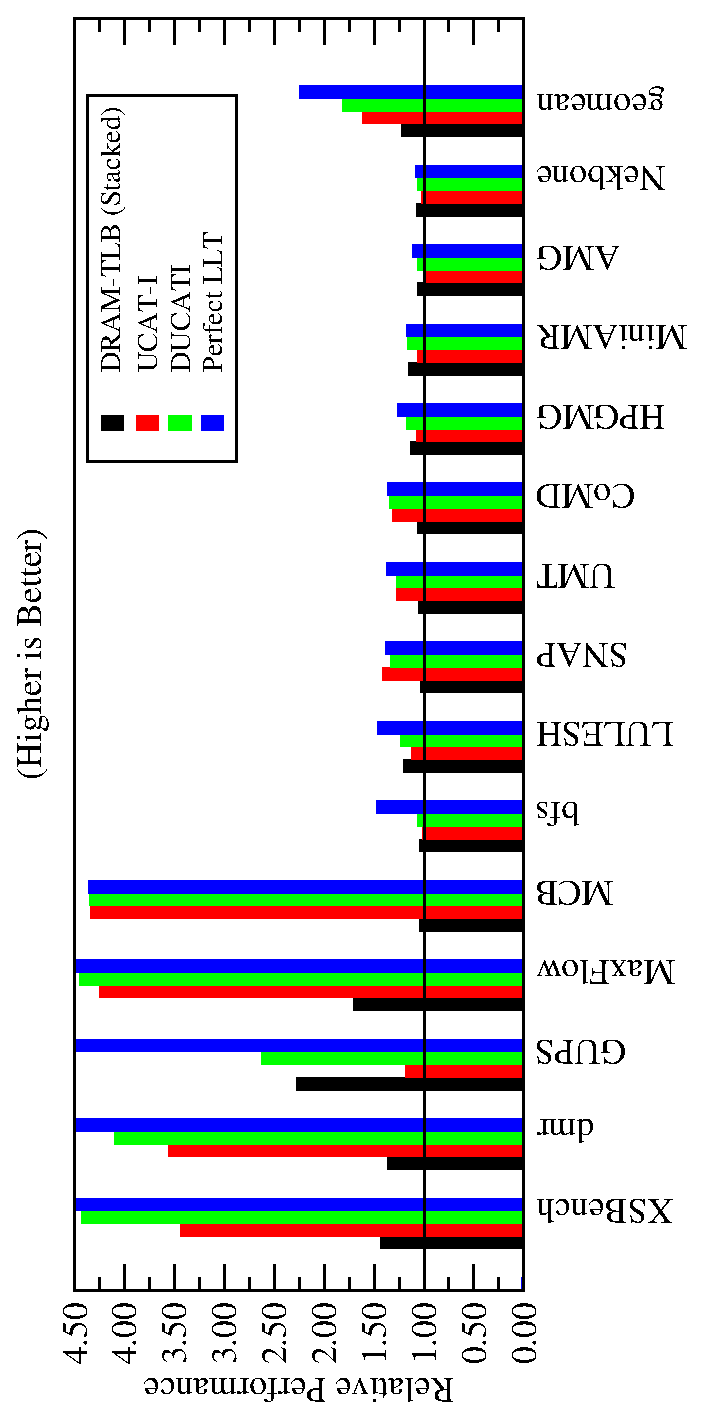
\psfig{file=GRAPHS/SUMMARY_perf,angle=-90,width=\columnwidth}}

\caption{\small Performance Summary (4KB page size).\normalsize}
\label{fig:summary_4k_pages_perf} 
\vspace{0.1 in}
\end{figure}

\begin{figure}[tp] 
\vspace{0.1 in} \centering
\centerline{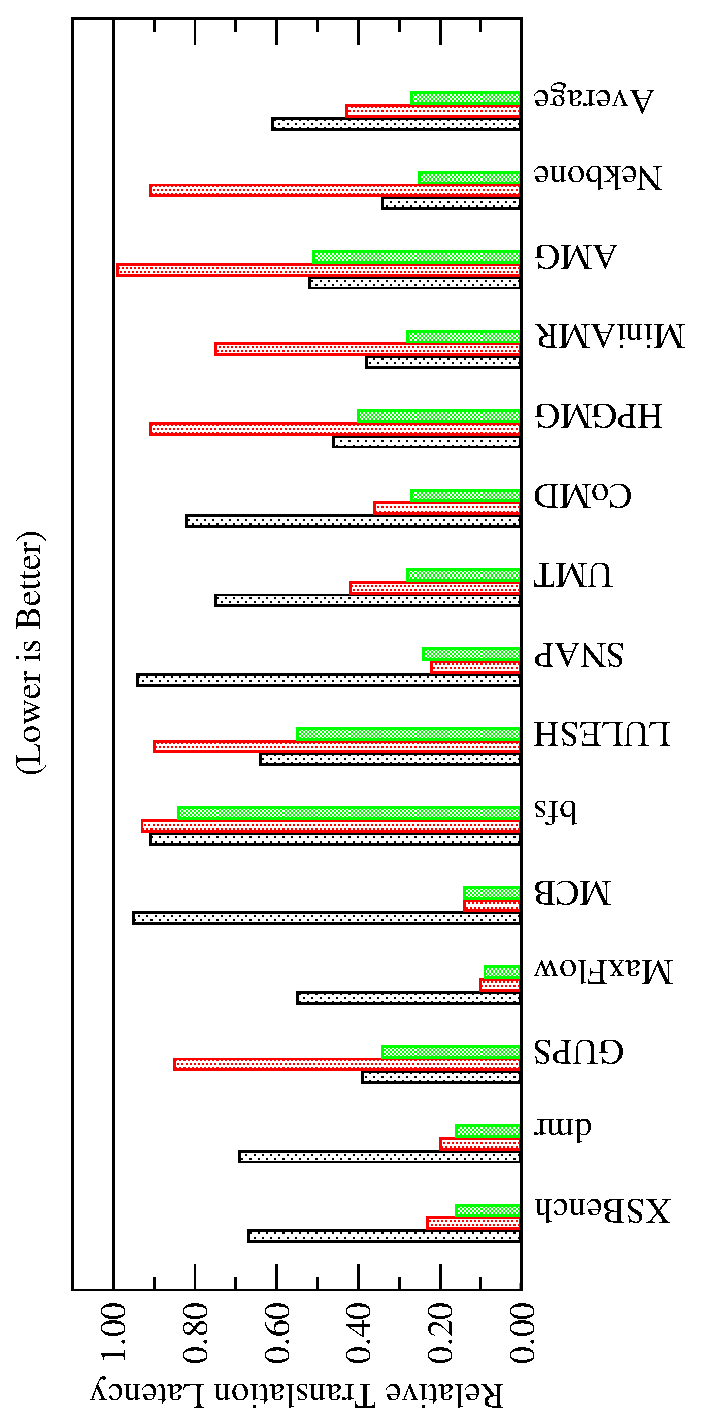
\psfig{file=GRAPHS/SUMMARY_tlblat,angle=-90,width=\columnwidth}}

\caption{\small Translation Latency (4KB page size) (same legend as
  Figure~\ref{fig:summary_4k_pages_perf}).\normalsize}
\label{fig:summary_4k_pages_lat} 
\vspace{-0. in}
\end{figure}

\noindent Figure~\ref{fig:summary_4k_pages_perf} illustrates the
relative performance of our proposals to the baseline system. The
x-axis shows the different workloads while the y-axis illustrates
performance. For each workload, we present the relative performance
for DRAM-TLBs architected with stacked memory (i.e. Stacked-TLB),
Unified Cache and TLB (UCAT) enhanced with insertion (UCAT-I), DUCATI,
and for comparison a hypothetical Perfect LLT system\footnote{We model
a Perfect LLT by assuming all references to the LLT in the baseline
system are hits}. To provide insight into the reason for performance
improvement, Figure~\ref{fig:summary_4k_pages_lat} presents relative
address translation latencies of the different proposals.

Figure~\ref{fig:summary_4k_pages_perf} shows that stacked memory
DRAM-TLBs improve average performance by 22\%, UCAT with insertion
(UCAT-I) improves average performance by 61\%, while DUCATI combines
the benefits of both to improve average performance by 81\%. In fact,
workloads like $XSBench$, $dmr$, $MaxFlow$, and $MCB$ experience 4x or
more performance improvement. The bulk of the gain for these workloads
is improvements in on-die LLT coverage. On the other hand, $GUPS$ has
a 2.5x performance primarily due to reduction in LLT miss penalty
(i.e., the DRAM-TLB component of DUCATI). For the medium and low TLB
sensitive workloads, DUCATI improves performance by 6-35\%.

Figure~\ref{fig:summary_4k_pages_lat} illustrates the relative address
translation latency for the different proposals. On average, DRAM-TLB
and UCAT reduce address translation latency by 40\% and 60\%
respectively, while DUCATI reduces address translation latency by
75\%. In doing so, DUCATI improves performance by 1.81x while a
perfect LLT system improves performance by 2.24x. Thus, DUCATI bridges
two-thirds of the performance gap between the baseline system and a
perfect LLT system.

% \ee{I don't see how 1.81x and 2.24x leads to 80\% of the performance
% gap being covered, it seems more like 64\% or something like that to
% me} 

% Note that Figure~\ref{fig:summary_4k_pages_lat} clearly identifies
% workloads that are are LLT capacity bound versus those workloads that
% are LLT miss penalty bound. Specifically, workloads where the first
% bar (DRAM-TLB) is lower than the second bar (UCAT) are those that
% limited by LLT miss penalty


\subsection{DUCATI Sensitivity to Page Size}

\noindent This section presents the performance of our proposals using
64KB and 2MB page sizes. For our 1024-entry baseline LLT, using 4KB
pages provides a TLB coverage of 4MB, using 64KB pages increases the
TLB coverage to 64MB, and using 2MB pages increases TLB coverage to
2GB. Note that while large page sizes improve TLB coverage,
unrestricted use of large pages can create various performance
overheads~\cite{SuperPageProblem,TwoPageSize,numa-harmful,cameo,largepagevm}.
Nonetheless, Figure~\ref{fig:summary_pagesize} illustrates the average
performance across all workloads for 4KB, 64KB, and 2MB pages.
Overall, DUCATI improves performance by 81\% with 4KB pages, 56\% with
64K pages, and 8\% with 2MB pages. In fact, DUCATI is within 20\%,
5\%, and 2\% the performance of an unrealistic perfect LLT system when
using 4KB, 64KB, and 2MB pages respectively. Thus, with both small and
large page sizes, DUCATI is able to significantly bridge gap between
the baseline system and a perfect LLT system.

\begin{figure}[tp] 
\vspace{0. in} \centering
\centerline{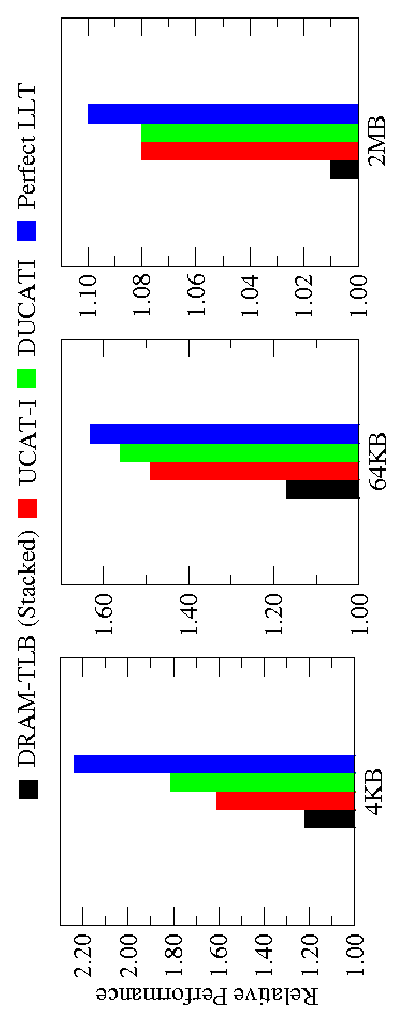
\psfig{file=GRAPHS/pagesize_sensitivity2,angle=-90,width=\columnwidth}}

\caption{\small Performance Sensitivity to Page Size (same legend as
Figure~\ref{fig:summary_4k_pages_perf}). \normalsize}

\label{fig:summary_pagesize} 
\vspace{-0. in}
\end{figure}

% \subsection{Sensitivity to Stacked DRAM Bandwidth}
% 
% \noindent Figure~\ref{fig:stack_bw_sense} illustrates the sensitivity
% of our proposals to stacked memory bandwidth. We evaluate four
% additional systems with 0.25X, 0.5X, 2X, and 4X the stacked memory
% bandwidth of the baseline system (we do not vary the system memory
% bandwidth). We increased the bandwidth by increasing the number of
% channels in the stacked memory system. The y-axis illustrates the
% average performance relative to the baseline system across all
% workloads in the study.
% 
% The figure shows that when the stacked memory bandwidth is plentiful,
% our proposals continue to improve performance. However, when the
% stacked memory bandwidth becomes a bottleneck, the memory queuing
% delays limit the performance of Distributed Placement. Under such
% scenarios, Stacked-TLBs still improve performance since they reduce
% the number of memory references. In general, our proposals efficiently
% utilize the spare bandwidth available in the stacked memory system.
% When the available bandwidth is high, performance improvements are
% high. When the available bandwidth is low, performance improvements

% % !TEX root = main.tex

% \begin {table*}[tp]
\small
\begin{center} 
\vspace{-0. in}
\caption{Summary of Distributed Placement and Stacked-TLBs for Different
Performance Metrics}
\vspace{-0. in}
\begin{tabular}{| c | c | c | c | c | }
\hline
Metric & Baseline & Distributed & Stacked-TLB & Perfect-LLT \\
       &          &  Placement  &             &             \\\hline
\# Page Table Lookups/LLT miss  & 1.75 & 1.75 & 1.00 &0.00 \\\hline
\multicolumn{5}{|c|}{ } \\ \hline
\multicolumn{5}{|c|}{ 4KB Page Size} \\ \hline
Throughput                            & 1.00 & 1.28 & 1.44 & 1.96 \\\hline
Relative LLT Miss Latency             & 1.00 & 0.70 & 0.51 & 0.00 \\\hline
Relative LLC Miss Latency             & 1.00 & 1.07 & 1.11 & 1.10 \\ \hline
\multicolumn{5}{|c|}{ } \\ \hline
\multicolumn{5}{|c|}{ 64KB Page Size} \\ \hline
Throughput                            & 1.00 & 1.04 & 1.12  & 1.34 \\\hline
Relative LLT Miss Latency             & 1.00 & 0.85 & 0.61  & 0.00 \\\hline
Relative LLC Miss Latency             & 1.00 & 1.03 & 1.05  & 1.07 \\ \hline

\end{tabular}
\label{table:results_summary}
\vspace{-0.015 in}
\end{center}
\normalsize
\end{table*}


\section{Results and Analysis} 
\label{sec:result}

\subsection{Results Summary}

\noindent Table~\ref{table:results_summary} summarizes several
performance metrics relative to the baseline system. Both Distributed
Placement and Stacked-TLB reduce LLT miss latency by 33\% and 49\%
respectively. The reduction in LLT miss latency improves performance
by 28\% and 44\% respectively. Stacked-TLB is best at reducing LLT
miss latency because the average page table accesses per LLT miss
reduce from 1.75 to a single Stacked-TLB access.

The table also shows that the different proposals tend to increase the
LLC miss latency by 7-10\%. This occurs because Distributed Placement
and Stacked-TLB both increase the traffic to stacked memory.
Consequently, the queuing delays in stacked memory increase. However,
the increase in LLC miss latency has minimal performance impact since
the large amount of memory-level parallelism present in these
workloads effectively hides the cache miss latency~\cite{bwa},

Figure~\ref{fig:summary_4k_pages} presents the per workload
performance behavior of Distributed Placement and Stacked-TLB relative
to a system with perfect LLT. The figure shows that distributed
placement bridges 30\% of the performance gap between the baseline
system and a perfect LLT while Stacked-TLB bridges 50\% of the
performance gap. In fact, for TLB-sensitive workloads like $CoMD$,
$BH$, $AMG\_2$, and $NEKBONE$ Stacked-TLB performs within 15\% of a
perfect LLT while using small page sizes.

\begin{figure}[tp] 
\vspace{-0 in} \centering
\centerline{\psfig{file=GRAPHS/4KB_pages_perf,angle=-90,width=\columnwidth}}

\caption{\small Performance with 4KB page size.\normalsize}
\label{fig:summary_4k_pages} 
\vspace{-0. in}
\end{figure}

\subsection{Sensitivity to Page Size}

\noindent We now present the performance of our schemes using 64KB
page size. For our 1024-entry baseline LLT size, using 64KB pages
increases the TLB coverage to 64MB (up to 256MB because of
~\cite{COLT}). In doing so, the LLT miss frequency reduces for
workloads that have high spatial locality in the virtual address
space. Table~\ref{table:results_summary} summarizes the different
performance metrics relative to the baseline system. With 64KB page
size, Distributed Placement and Stacked-TLB reduce LLT miss latency by
15\% and 39\% respectively. In turn, they improve performance by 4\%
and 12\% respectively.

With 64KB page size, Figure~\ref{fig:summary_64k_pages} presents the
per workload performance behavior of our baseline system, Distributed
Placement and Stacked-TLB relative to a perfect LLT system. We observe
that workloads with high spatial locality within a 64KB page tend to
observe fewer LLT misses. Consequently, the baseline system itself is
within 30\% of a perfect LLT (as opposed to 50\% for the 4KB page size
system). However, there is still opportunity to improve performance of
workloads that are TLB-sensitive with 64KB pages (e.g. $HPGMG$, $DMR$,
and $XSBENCH$). For these workloads, Distributed Placement and
Stacked-TLB proposals improve performance by 27-45\%. Overall,
Stacked-TLB bridges 30\% of the performance gap between the baseline
system and a perfect LLT.


% However, for workloads with limited
% spatial locality in a 64KB page (e.g. HPGMG, DMR) still benefit from
% our proposals.
% 
% We show that that distributed pagetable placement improves performance
% by 4\% while DRAM-TLBs and Stacked-TLBs improve performance by 14\%
% and 11\% respectively. We find the performance benefits from
% distributed page table placement diminishing with increasing page
% size. This is beacause fewer LLT misses cause the average number of
% memory requests to the memory system to increase. Since the majority
% of requests are serviced by the stacked memory, increasing queuing
% delays take away any benefit realized from page table placement. 
% 
% We note that it is exactly for this reason that DRAM-TLBs also
% outperform Stacked-TLBs at times. Since the majority of requests are
% serviced by stacked memory, average stacked memory access latency can
% be longer than the average system memory access latency (at least
% until system memory bandwidth saturates).

\begin{figure}[tp] 
\vspace{0. in} \centering
\centerline{\psfig{file=GRAPHS/64KB_pages_perf,angle=-90,width=\columnwidth}}

\caption{\small Performance with 64KB page size.\normalsize}

\label{fig:summary_64k_pages} 
\vspace{-0. in}
\end{figure}

\subsection{Sensitivity to Stacked DRAM Bandwidth}

\noindent Figure~\ref{fig:stack_bw_sense} illustrates the sensitivity
of our proposals to stacked memory bandwidth. We evaluate four
additional systems with 0.25X, 0.5X, 2X, and 4X the stacked memory
bandwidth of the baseline system (we do not vary the system memory
bandwidth). We increased the bandwidth by increasing the number of
channels in the stacked memory system. The y-axis illustrates the
average performance relative to the baseline system across all
workloads in the study.

The figure shows that when the stacked memory bandwidth is plentiful,
our proposals continue to improve performance. However, when the
stacked memory bandwidth becomes a bottleneck, the memory queuing
delays limit the performance of Distributed Placement. Under such
scenarios, Stacked-TLBs still improve performance since they reduce
the number of memory references. In general, our proposals efficiently
utilize the spare bandwidth available in the stacked memory system.
When the available bandwidth is high, performance improvements are
high. When the available bandwidth is low, performance improvements
are low.

\begin{figure}[t] 
\vspace{0.1 in} \centering
\centerline{\psfig{file=GRAPHS/sensitivity_stack_bw,angle=-90,width=\columnwidth}}

\caption{\small Sensitivity to stacked memory bandwidth. \normalsize}
\label{fig:stack_bw_sense} 
\vspace{-0 in}
\end{figure}


% \newpage
\section{DUCATI Discussion } 
\label{sec:implications}

% \subsection{Performance Impact On CPUs}
% 
% \noindent Our baseline studies assume on-die integrated CPU-GPU
% systems~\cite{intelgen9, amdzen} with a hybrid memory system. On such
% systems, both the GPU and CPU have similar access latency to both the
% stacked memory and system memory. While our have studies focused
% primarily on GPU workloads, both Page Table Placement and Stacked-TLB
% proposals are also expected to improve the performance of
% TLB-sensitive CPU workloads.
% 
% Our proposals also apply to discrete CPU-GPU systems where the CPU and
% GPU communicate using high speed links (e.g. QPI~\cite{intel_qpi},
% NVLink~\cite{bwa}). In commercially offered discrete systems
% today~\cite{hbm_intel, hbm_nvidia}, stacked memory is normally
% integrated on the GPU while system memory is normally integrated on
% the CPU. Thus, the GPU/CPU experiences longer unloaded access latency
% to the remote non-integrated memory (due to the additional round trip
% communication link latency).
% 
% Since the GPU is directly connected to the stacked memory on discrete
% CPU-GPU systems, the GPU continues to benefit from our stacked memory
% proposals to improve address translation. A natural question is how
% our proposals affect CPU performance on discrete CPU-GPU systems? At
% first, it may seem that our stacked memory proposals will degrade CPU
% performance because the unloaded access latency to stacked memory is
% longer than to the baseline system memory. However, CPU performance
% behavior depends on the bandwidth utilization and observed latency to
% system memory.
% 
% When system memory bandwidth is saturated, the stacked memory access
% latency tends to be lower than the observed system memory access
% latency. In fact, our studies revealed a 10\% lower stacked memory
% latency from the CPU relative to accessing the system memory. This is
% despite including the round trip communication link latency. As such,
% we expect our proposals to also improve CPU performance on discrete
% CPU-GPU system when the system memory bandwidth is saturated.
% 
% In situations where the system memory bandwidth is not saturated, we
% can ensure no impact on CPU performance, by always applying the
% baseline policy for CPU workloads. For example, the operating system
% can always follow System Memory Placement for all CPU workloads.
% Furthermore, the CPU can always follow the baseline policy of walking
% the page table when it misses in its own last level TLB, rather than
% probing the Stacked-TLB. A dynamic decision may be possible where the
% CPU can adapt to either using the baseline policy or our stacked
% memory proposals depending on the bandwidth utilization of system
% memory. We leave these optimizations for future work.
% 
\subsection{Performance Impact on VM Operations}

\noindent Virtual memory operations such as remapping the virtual to
physical address or changes to page permissions require sending page
table update requests and TLB shootdowns to stacked memory in both the
Distributed Page Table Placement and Stacked-TLB proposals. One
potential concern is whether the stacked memory access latency can
impact the overall latency of these virtual memory operations. 

The virtual memory operations discussed above normally occur as a part
of a CPU generated interrupt flow which ranges from 5-30
microseconds~\cite{zhengpagedgpu}. The observed access latency for
stacked memory across all our workloads tends to be 100-250
nanoseconds . Thus, even in the worst case, the stacked memory access
latency is a small fraction of the overall interrupt latency (2-5\%).
Realistically, when the system memory bandwidth is saturated, we
expect performance improvements relative to the baseline system since
the observed stacked memory access latency would be significantly
lower than the observed system memory access latency. As such, we
expect our stacked memory proposals to have negligible performance
impact on VM operations.

% Though DRAM-TLB shootdowns and flush events consume bandwidth, these
% events occur infrequently and thus we expect minimal performance
% impact.

% TLB shootdowns can either be implemented either by performing a
% DRAM-TLB lookup and address comparison or simply by zeroing the
% DRAM-TLB-entry without reading its contents. On the other hand, the
% hardware overhead for flushing a DRAM-TLB is equivalent to
% initializing a large region of memory.
% 


%!TEX root=main.tex
\section{Related Work}

\noindent While significant literature exists on improving TLB
performance, we discuss recent work that is most closely related to
the work described in this paper.

\boldheadingpara{Improving TLB Performance} Recent papers improve TLB
coverage through compression~\cite{COLT, tlbreachclustering} and
enhanced TLB organizations~\cite{SharedLLT, simTLBperf} by changing
the existing TLB structures. Other work has investigated mechanisms to
accelerate page walks by caching portions of the page
table~\cite{SkipPT,MMUcaches}, or prefetching TLB
entries~\cite{prefTLBintercore, prefTLBgokul, prefTLBrecency,
power2014supporting}, or speculating on the address translation on TLB
misses~\cite{spectlb}. When the memory footprint of workloads is
extremely large, such proposals are unable to provide full TLB
coverage and avoid TLB miss overhead. Our work focuses both on
increasing TLB coverage and reducing TLB miss penalty by storing TLB
entries in the conventional LLC and embedding a TLB in DRAM. DRAM-TLB
skips the page walk entirely and in the common case provide address
translations using a single memory access.

\boldheadingpara{Large Pages and Direct Segments} Our studies show
that the use of large pages (e.g. 2MB, 64MB, 1GB) and direct
segments~\cite{Basu2013} can significantly improve TLB coverage.
However, recent work has shown that unrestricted use of large pages
creates unintended performance
overheads~\cite{SuperPageProblem,TwoPageSize,numa-harmful,cameo,largepagevm}
causing modern operating systems to avoid using large pages in the
common case. Alternatively, the use of direct segments can improve TLB
coverage. However, direct segments requires both hardware and software
support to redesign the existing address translation system. Our
proposals on the other hand provide a complementary approach to
improve address translation using smaller pages (4KB, 64KB) without
the overhead of large pages and the design complexity of direct
segments. 

\boldheadingpara{Alternate DRAM Architectures} Recent proposals extend
the processor cache hierarchy by architecting stacked memory as a DRAM
cache~\cite{BEAR, moin2012, unison, loh2011, jaewoong2012,
dramcache-resilient}. The trade-offs for architecting DRAM-TLBs are
different from those considered in DRAM cache designs. For example,
DRAM-TLB entries are much smaller than DRAM cache entries and as such,
DRAM-TLBs expose different trade-offs for reading and updating
multiple entries without incurring higher latency or bandwidth. 
Overall, DRAM caches are orthogonal to the proposals of
this paper.

\boldheadingpara{Data Placement in Hybrid Memory} Application data
placement in hybrid memory systems as well as NUMA system has been
well studied. Hybrid memory placement policies attempt to fully
utilize total system bandwidth by distributing pages between system
memory and stacked memory based on the bandwidth
ratio~\cite{bwa,batman}. NUMA aware placement on the other hand
focuses on data placement near computing resources to minimize overall
latency~\cite{numa-traffic, numa-OSsupport, numa-bolosky}. Our work is
orthogonal these proposals.

\boldheadingpara{Address Translation Support for GPUs} Efficient and
high performing address translation on GPUs is an important area of
research. Recent studies~\cite{power2014supporting, pichaigpu} show
that simply extending CPU-style TLBs and page walkers to GPUs do not
perform well. Consequently, novel mechanisms such as highly threaded
page walkers~\cite{power2014supporting} and intelligent page walk
scheduling~\cite{pichaigpu} have been proposed. Our work focuses on
improving GPU TLB coverage by allowing the GPU LLC to hold TLB
entries. Additionally, we improve GPU TLB miss latency by architecting TLBs in DRAM.

\boldheadingpara{Inverted Page Tables} To reduce the number of memory
accesses in a hierarchical page table design, some designs use
inverted page tables~\cite{invertedPT,invertedPT2}. Inverted page
tables are designed to provide translation with a single memory access
by indexing the page table using a hash of the virtual address.
However, since different virtual addresses might produce a similar
hash, a collision-chain is created. Consequently, a drawback is that
the number of memory accesses is dependent on the length of the
collision chain. Another drawback of inverted page tables with respect
to hierarchical page tables is that they do not allow simultaneous
mapping of two different virtual addresses to the same physical
address~\cite{invertedPT}. DRAM-TLBs target the same benefits of
inverted page tables (i.e., address translation in a single memory
access) while retaining the benefits of hierarchical page tables.

% \ee{This section is pretty
% entertaining. First of all, there is no citation so its not clear what
% prior work we're even talking about. Second, it is just right out the
% gates telling the world how shitty inverted page tables are!!! I think
% a beginning sentene telling the reader why we're even talking about
% inverted page tables and also giving a citation to the related work is
% in order.} 


% DRAM-TLBs leverage the hierarchical page table structure
% and allow shared address spaces. Inverted page tables on the other
% hand do not allow shared spaces. Second, inverted page tables rely on
% a hash function to search the page table. In case of conflicts, a
% linked list must be traversed to find the translation. As such
% inverted page tables may require more than one memory access. On the
% other hand, 

% DRAM-TLBs in most common case yields a translation in a single lookup.
% However, inverted page tables first require a hash function to
% determine where to start the search, and then a linked list traversal
% to the find the corresponding mapping. Additionally, unlike inverted
% page tables, DRAM-TLBs allow flexible share of data between multiple
% virtual addresses/processes.

%!TEX root=main.tex
\section{Summary}

\noindent Increasing application memory footprints and growing on-die
thread-level parallelism has made TLB performance an important
performance bottleneck in today's systems. Even page walk caching
mechanisms are unable to accommodate emerging application working-set
sizes. As a result, Last-Level TLB (LLT) coverage can be very
important to overall application performance. On the other hand LLT
misses suffer long latency due to multiple memory accesses to the page
table. As such, when LLT misses occur, reducing address translation
latency is necessary to maintain high performance.

This paper proposes low-cost hardware mechanisms to accelerate virtual
to physical address translation by improving on-die {\em LLT coverage}
and {\em LLT miss penalty}. We improve on-die TLB coverage by
proposing {\em Unified Cache and TLB (UCAT)}, which enables the
conventional unified Last-Level Cache (LLC) to also hold TLB entries.
UCAT increases on-die LLT coverage by allowing as many TLB entries as
there are cache lines in the conventional on-chip LLC. We show that
UCAT improves performance by 60\% (up to 4x) on average across a set
of memory intensive GPU workloads. We show that these improvements can
be realized with negligible changes to the existing LLC architecture.

% This is because it still requires multiple requests to the page table
% for retrieving the address translation.

While UCAT improves performance significantly, it does not decrease
the number of page table accesses on an LLT miss. To address this
problem, we propose {\em DRAM-TLB}. DRAM-TLB serves as the next larger
level in the TLB hierarchy architected in DRAM technology and can be
arbitrarily sized to provide the desired TLB coverage. In steady
state, DRAM-TLB can avoid multiple page table accesses and provides
address translation using a single memory access. Consequently,
DRAM-TLB is a low latency alternative to walking the page table on an
LLT miss. Our studies show that DRAM-TLB architected using stacked
memory technology improves performance by 22\% on average (up to
2.25X). We show that DRAM-TLB requires less than 1\% the capacity of
our baseline 16GB stacked memory system.

Finally, we propose {\em DUCATI}, an address translation architecture
that combines the benefits of DRAM-TLBs and UCAT while requiring
negligible hardware overhead. DUCATI improves performance by 81\% (up
to 4.5x) for 4KB pages and by 56\% and 8\% when applied to 64KB and
2MB page systems respectively.

% \newpage
% We have shown that emerging stacked memory technologies have now
% enabled a new TLB architecture previously was not practical with
% commodity DRAM. Since Stacked-TLBs enable high TLB coverage, we hope
% that they can spur future research directions in areas where
% extracting TLB performance has been challenging (e.g. virtualization).
% 


\begin{small}
%\bibliographystyle{ieeetr}
\bibliographystyle{IEEEtranS}
\bibliography{sigproc}
\end{small}
%%%%%%%%%%%%%%%%%%%%%%%%%%%%%%%%%%%%%%%%%%%%%%%%%%%%%%%%%%%%%%%%%%%%%%%%%%%%%%%%%%%%%%%%%%%%%%%

\end{document}
